%!TEX ROOT = thesis.tex

\chapter{Semantics Retrieval Engine, Results and Analysis}

\label{section:retrievalengine}
\section{Introduction}

As described in Section~\ref{section:introduction}, there's an evident gap between the process of obtaining user described events and the retrieval of the desired video shots. Traditional approach of collecting text-based description of events alone are insufficient for effective retrieval process.
With vehicle-specific semantics such as vehicle trajectory, time-stamp information, and colour information extracted via the extraction module introduced in Chapter~\ref{section:semanticsextraction},
this chapter hone in on the second objective [02] of designing video retrieval techniques that takes in intuitive user-described queries to provide fast and accurate results.

To this end, a combination of keyword and sketch based retrieval engine was designed for end users to describe their queries intuitively.
First, the design choices of the semantic retrieval engines are engaged in detail. Two retrieval techniques with relatively different concepts and underlying frameworks were designed.
The first technique was designed with a classic document retrieval system in mind, inspired by Locality Sensitive Hashing (LSH), while the second technique was developed in order to address the shortcomings of the first by introducing similarity scores obtained using Chamfer Distance.

Subsequently, the methods used to measure the difference between the user-described trajectory, vehicle colour classifying methods, scoring systems along with the results based on multiple users' review of the proposed method is discussed.
As described in the Experimental Methodology (see~\ref{sec:expmethodology}), both the vehicle trajectory and vehicle colour evaluation process were separated in order to better gauge the performance of each technique.
This chapter also includes the retrieval speed of the second retrieval engine.
Furthermore, the evaluation and analysis of their performances along with the metrics used are further discussed. This chapter concludes with some suggestions for future improvements.

\section{\versionOneRet}
\label{section:versionOne}
This section uncovers the techniques used behind this retrieval engine's framework along with the results. As previously introduced, this retrieval engine was inspired by Locality Sensitive Hashing (LSH) where documents are hashed into similar locations depending on the similarity. With that in mind,  the concept of this retrieval engine is first discussed. Next, the scoring system is introduced followed by the evaluation of the system in the following subsections.

\subsection{Concept}
\label{versionOneConcept}
By taking advantage of the spatio-temporal atom cubes structure introduced in Chapter~\ref{section:atoms}, each catalogued event in an atom was treated as a unique document. The underlying atom-based structure allows queries to be formed in a way which emulates the semantics extraction process. Hence, eliminating the need for query parsing which in turn reduces the required computational time.

In this setup, each document containing similar contents were placed in the same SQL table as a mode of clustering documents. An example is given in Table~\ref{table:dbSample} to provide better visualisation of the proposed method. These sequence of events is also visualised in Figure~\ref{fig:motionExample} with the trajectory marked with \textcircled{2}.
In the example, a red vehicle was detected frame 180 to 184 of a video file on the 19th of March 2016 at 8:51:00am until 8:51:05am, from atom location (3, 15) to (5, 17) but was detected as a pink vehicle at frame 181.
The time information from frame $\mathbb{T}$ can be deduced using $\mathbb{T}_{time}  = (\mathbb{VD} \times \frac{\mathbb{T}}{\mathbb{TF}}) + \mathbb{F}_{time}$ where $\mathbb{VD}$ corresponds to the video duration of each file (6 minutes) and $\mathbb{TF}$ is the total frames of the current video. The $\mathbb{F}_{time}$ is the time information extracted from filename.
Hence, the current frame time at frame 181 is obtained as such: $(6_{minutes} \times \frac{181}{360}) + 08:48:00am = 8:51:01am$.

As each catalogued event is treated as a unique document (a single record in the database) in this framework, the retrieval process begins by filtering out tables which are irrelevant to the query, $\mathbb{Q}$. Falling back on the example given in Table~\ref{table:dbSample}, the system is able to effectively skip through 9 colour tables and 5 motion tables, hence speeding up the process of locating documents of interest while reducing the overhead cost involved when going through an entire database. Upon filtering out irrelevant tables, the retrieval engine proceeds to extract and group up all the relevant records according to the filenames.

Next, the retrieved results are validated to see if they belong to the same vehicle by cross-checking the obj\_id. Along with that, the retrieval engine also validates if the results belong to a similar time-frame by comparing the t-coordinate. This step is essential to ensure that each result belongs to the same vehicle trajectory group as the initial tracker may re-assign a obj\_id to another vehicle during the background subtraction process.
Although the results returned at this point are moderately accurate, one major problem that occurs using the current process is the low recall rate. The recall rate in a retrieval engine can be thought as the percentage of relevant documents retrieved over the total amount of relevant documents available in the database. While low recall rates might be preferable in an environment where the accuracy of the retrieved result is of higher importance and false negatives are welcomed over false positive such as the medical industry, this is not the case in the proposed method.

To overcome the limitation of low recall rates, a Confidence Value (CV) score parameter is introduced to adjust the sensitivity level of accepting a video shot as part of the final retrieved results. In the proposed method, a lower CV would return larger set of results at the expense of an increase of retrieved shots which may or may not improve the overall accuracy. Each retrieved shot, $\mathbb{S}_i$, will be accepted as the final retrieved results if it fulfils the condition in Equation \ref{eq:CVscore}. The use of the CV score parameter provides a margin of error when performing the query which acts as a trade-off function.

\begin{equation}
\label{eq:CVscore}
CV < \frac{\text{length}(\mathbb{S}_i)}{\text{length}(\mathbb{Q})} \times 100\%
\end{equation}

Upon validating the sanctity of the results, commands were sent to FFmpeg to extract the video shots based on the given filename along with the start and end frame number. Finally, the users are presented with the output from the retrieval engine where the final results can be viewed.


% Please add the following required packages to your document preamble:
% \usepackage[normalem]{ulem}
\begin{table}[!hbt]
	\centering
\caption{Database Structure for a Vehicle Identified as Red and Pink Colour with Object id "1" of the \versionOneRet }
\label{table:dbSample}
\begin{tabular}{llllll}
\multicolumn{6}{l}{{ colour\_red}} \\ \hline
\multicolumn{1}{|l|}{\textbf{row\_id}} & \multicolumn{1}{l|}{\textbf{filename}}    & \multicolumn{1}{l|}{\textbf{obj\_id}} & \multicolumn{1}{l|}{\textbf{atom\_x}} & \multicolumn{1}{l|}{\textbf{atom\_y}} & \multicolumn{1}{l|}{\textbf{atom\_t}} \\ \hline
\multicolumn{1}{|l|}{n}                & \multicolumn{1}{l|}{20160319\_084800.mp4} & \multicolumn{1}{l|}{1}                & \multicolumn{1}{l|}{3}                & \multicolumn{1}{l|}{15}               & \multicolumn{1}{l|}{180}              \\ \hline
\multicolumn{1}{|l|}{n+1}              & \multicolumn{1}{l|}{20160319\_084800.mp4} & \multicolumn{1}{l|}{1}                & \multicolumn{1}{l|}{3}                & \multicolumn{1}{l|}{16}               & \multicolumn{1}{l|}{182}              \\ \hline
\multicolumn{1}{|l|}{n+2}              & \multicolumn{1}{l|}{20160319\_084800.mp4} & \multicolumn{1}{l|}{1}                & \multicolumn{1}{l|}{4}                & \multicolumn{1}{l|}{16}               & \multicolumn{1}{l|}{183}              \\ \hline
\multicolumn{1}{|l|}{n+3}              & \multicolumn{1}{l|}{20160319\_084800.mp4} & \multicolumn{1}{l|}{1}                & \multicolumn{1}{l|}{5}                & \multicolumn{1}{l|}{17}               & \multicolumn{1}{l|}{184}              \\ \hline
                                       &                                           &                                       &                                       &                                       &                                       \\
\multicolumn{6}{l}{{ colour\_pink}}                                                                                                                                                                                                              \\ \hline
\multicolumn{1}{|l|}{\textbf{row\_id}} & \multicolumn{1}{l|}{\textbf{filename}}    & \multicolumn{1}{l|}{\textbf{obj\_id}} & \multicolumn{1}{l|}{\textbf{atom\_x}} & \multicolumn{1}{l|}{\textbf{atom\_y}} & \multicolumn{1}{l|}{\textbf{atom\_t}} \\ \hline
\multicolumn{1}{|l|}{m}                & \multicolumn{1}{l|}{20160319\_084800.mp4} & \multicolumn{1}{l|}{1}                & \multicolumn{1}{l|}{3}                & \multicolumn{1}{l|}{16}               & \multicolumn{1}{l|}{181}              \\ \hline
                                       &                                           &                                       &                                       &                                       &                                       \\
\multicolumn{6}{l}{{ direction\_down}}                                                                                                                                                                                                          \\ \hline
\multicolumn{1}{|l|}{\textbf{row\_id}} & \multicolumn{1}{l|}{\textbf{filename}}    & \multicolumn{1}{l|}{\textbf{obj\_id}} & \multicolumn{1}{l|}{\textbf{atom\_x}} & \multicolumn{1}{l|}{\textbf{atom\_y}} & \multicolumn{1}{l|}{\textbf{atom\_t}} \\ \hline
\multicolumn{1}{|l|}{h}                & \multicolumn{1}{l|}{20160319\_084800.mp4} & \multicolumn{1}{l|}{1}                & \multicolumn{1}{l|}{3}                & \multicolumn{1}{l|}{15}               & \multicolumn{1}{l|}{181}              \\ \hline
                                       &                                           &                                       &                                       &                                       &                                       \\
\multicolumn{6}{l}{{ direction\_motionless}}                                                                                                                                                                                                    \\ \hline
\multicolumn{1}{|l|}{\textbf{row\_id}} & \multicolumn{1}{l|}{\textbf{filename}}    & \multicolumn{1}{l|}{\textbf{obj\_id}} & \multicolumn{1}{l|}{\textbf{atom\_x}} & \multicolumn{1}{l|}{\textbf{atom\_y}} & \multicolumn{1}{l|}{\textbf{atom\_t}} \\ \hline
\multicolumn{1}{|l|}{j}                & \multicolumn{1}{l|}{20160319\_084800.mp4} & \multicolumn{1}{l|}{1}                & \multicolumn{1}{l|}{3}                & \multicolumn{1}{l|}{16}               & \multicolumn{1}{l|}{182}              \\ \hline
                                       &                                           &                                       &                                       &                                       &                                       \\
\multicolumn{6}{l}{{ direction\_right}}                                                                                                                                                                                                         \\ \hline
\multicolumn{1}{|l|}{\textbf{row\_id}} & \multicolumn{1}{l|}{\textbf{filename}}    & \multicolumn{1}{l|}{\textbf{obj\_id}} & \multicolumn{1}{l|}{\textbf{atom\_x}} & \multicolumn{1}{l|}{\textbf{atom\_y}} & \multicolumn{1}{l|}{\textbf{atom\_t}} \\ \hline
\multicolumn{1}{|l|}{k}                & \multicolumn{1}{l|}{20160319\_084800.mp4} & \multicolumn{1}{l|}{1}                & \multicolumn{1}{l|}{3}                & \multicolumn{1}{l|}{16}               & \multicolumn{1}{l|}{183}              \\ \hline
                                       &                                           &                                       &                                       &                                       &                                       \\
\multicolumn{6}{l}{{ direction\_right\_down}}                                                                                                                                                                                                   \\ \hline
\multicolumn{1}{|l|}{\textbf{row\_id}} & \multicolumn{1}{l|}{\textbf{filename}}    & \multicolumn{1}{l|}{\textbf{obj\_id}} & \multicolumn{1}{l|}{\textbf{atom\_x}} & \multicolumn{1}{l|}{\textbf{atom\_y}} & \multicolumn{1}{l|}{\textbf{atom\_t}} \\ \hline
\multicolumn{1}{|l|}{l}                & \multicolumn{1}{l|}{20160319\_084800.mp4} & \multicolumn{1}{l|}{1}                & \multicolumn{1}{l|}{3}                & \multicolumn{1}{l|}{16}               & \multicolumn{1}{l|}{184}              \\ \hline
\end{tabular}
\end{table}

\subsection{Search Interface}

The proposed retrieval engine was presented in a graphical user search interface written in C++. Here, users are able to construct queries by drawing the trajectory on the search interface while providing complementary query information such as the vehicle colour. With these user-described query information, the retrieval engine would search for the best matches and return the results within seconds. Figure \ref{fig:versionOneInterface} shows the proposed interface with the green lines indicating the user-described trajectory query. Upon processing the results, FFmpeg will then extract the video shots and populate the results in a folder.


\begin{figure}[!htb]
	\centering
	\begin{tabular}{c}
		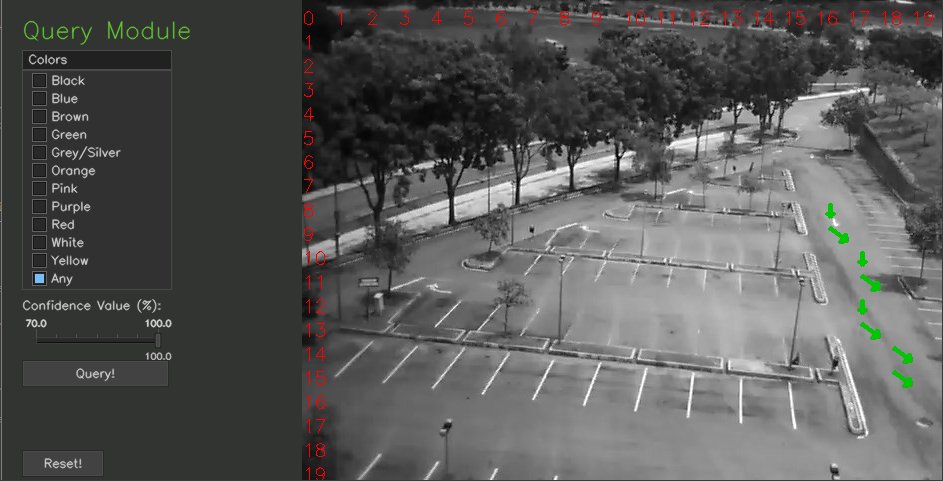
\includegraphics[width=0.7\linewidth]{image/retrievalOne/test1-8inputs.PNG} \\
		(a) Motion Test Case 1 (TQ1) \\
		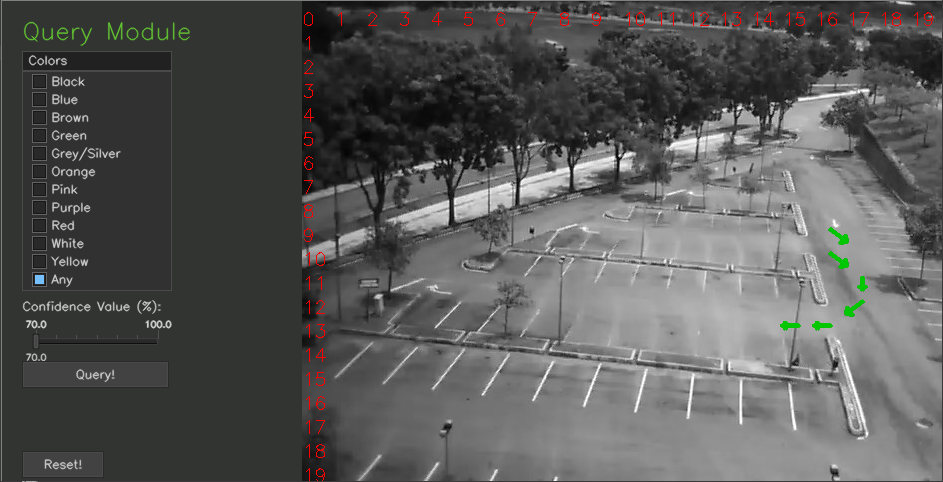
\includegraphics[width=0.7\linewidth]{image/retrievalOne/test2-6input.PNG}\\
		(b) Motion Test Case 2 (TQ2)
	\end{tabular}
	\caption{Search Interface for \versionOneRet}
	\label{fig:versionOneInterface}
\end{figure}


\subsection{Results and Analysis}
The following subsections describes the evaluation process of the proposed method in Section \ref{section:semantic_lsh} which includes both the vehicle trajectory as well as the vehicle colour. As previously mentioned in Section \ref{sec:expmethodology}, only two days of data were fully annotated with the number of vehicles with their corresponding colour (see Table \ref{table:colorDist}) as well as the total number of vehicles that performed both $TQ1$ and $TQ2$.

Precision and Recall (Equation \ref{eq:precisionrecall}) metrics were used to measure the performance of the proposed method. These values can be calculated as the total number of event occurrence for 2 days were fully annotated. Likewise, as the $F_1$ score is a harmonic mean between Precision and Recall, this value can also be computed (Equation \ref{eq:f1score}). The precision of a retrieval engine can be thought as the ratio between number of accurate results over the total number of retrieved results. The recall, on the hand, indicates the ratio of relevant results which were retrieved over the total retrieved results. As both Precision and Recall values are desirable in a retrieval engine, the $F_1$ score is used to judge how well the retrieval engine performs in these two aspects.

\begin{align}
\label{eq:precisionrecall}
    \text{Precision} = \frac{tp}{tp + fp}   \hspace{1em} \text{ ; }  \hspace{1em} \text{Recall}  = \frac{tp}{tp + fn}
\end{align}
\begin{align}
\label{eq:f1score}
\text{F1-score}  = 2\cdot\frac{\text{Precision} \cdot \text{Recall}}{\text{Precision} + \text{Recall}}
\end{align}


\subsubsection{Vehicle Trajectory}

To evaluate the performance of the proposed method in retrieving vehicle trajectories, the ground truth of the data has to be first obtained. As the manual annotation of these video data is laborious and time consuming, only two specific motion paths were designated as trajectory queries (TQ). The first query, TQ1 refers to vehicles heading southward (see Figure \ref{fig:versionOneInterface} (a)) while TQ2 represents vehicles turning into a junction (see Figure \ref{fig:versionOneInterface} (b)).

These predefined trajectory queries (TQ) were selected to represent two types of motion which are common in a typical car park scene, (i) \textit{simple motion} - motions that are simple in nature, moving straight \& (ii) \textit{complex motion} - motions which contains two or more motion elements such as turning into a junction. The distribution of these TQ are tabulated in Table \ref{table:motiondist}. In each TQ experiment, the number of atom selected in the input queries were varied to understand the relation between the number of inputs and the performance of the retrieval engine. In addition, the effects of using varying confidence values (CV) was also evaluated. These experiments were tested on three CV values which were set at 70\%, 80\%, and 90\%.


\begin{table}[bht!]
\centering
\caption{Ground Truth Distribution of Trajectory Queries}
\label{table:motiondist}
\begin{tabular}{cccc}
\toprule
Trajectory Query &  Trajectory Type & \# of Occurrence & Distribution (\%)   \\
\midrule
TQ1       & Simple Motion       & 252 & 86.3   \\
TQ2      & Complex Motion       & 40 & 13.7  \\
\bottomrule
\end{tabular}
\end{table}

Based on the results tabulated in Table \ref{table:motionResults}, the average precision of both TQ1 and TQ2 using CV at 70\% is 67.64\%. The increase of CV to 70\% to 90\% shows an increase in terms of average precision. For TQ1, the average precision increased from 89.50\% to 90.49\% when CV was set at 90\% with a total increase of approximately 1\%. However for TQ2, the average precision showed a sizeable improvement of 7.44\% when then CV parameter was tweaked. The average precision increased from 45.79\% to 53.23\% when CV was set to 90\%.
However, as expected, the recall metrics showed a different side of the story when the average recall rate suffered a drastic drop from 39.67\% to 18.01\% for TQ1 and 68.15\% to 51.85\% for TQ2. The results shows consistency throughout the various experimental settings and true towards the concept which was introduced in \ref{versionOneConcept}.

To judge the overall performance of the retrieval engine as a whole, the $F_1$ score metric was used as it provides a harmonic mean between both of the desirable metrics discussed above. Based on the results, queries with the lowest CV and lower number of inputs tend to perform better than the other parameter settings.
This is because the additional number of input increases the chance of lowering the CV score; likewise, a lower CV value relaxes the need to match more atom inputs.
The proposed method was able to achieve an $F_1$ score of 74.32\% and 68.08\% for both TQ1 and TQ2.
Based on the results obtained from these experiments, the performance of the proposed method was far from optimal. Drastic changes are inevitable if improvements is desired. The changes in the proposed method will be further discussed in Section \ref{section:versionTwo}.


\begin{table}[tb!]
\centering
\caption{Results of Motion Retrieval Task with Varying CV and Number of Atom Inputs}
\label{table:motionResults}
\vspace{0.5em}
\resizebox{\textwidth}{!}{
\begin{tabular}{ccc|c|c|c|c|c|c|c|c|c|}
\cline{4-12}
\cline{4-12}
& & & \multicolumn{3}{c|}{CV: 70\%} & \multicolumn{3}{c|}{CV: 80\%} & \multicolumn{3}{c|}{CV: 90\%} \\ \cline{4-12}
 & & & Precision & Recall & F1 Score & Precision & Recall & F1 Score & Precision & Recall & F1 Score \\ \hline
\multicolumn{1}{|c|}{\multirow{7}{*}{\rotatebox[origin=c]{90}{No. of Input}}} & \multicolumn{1}{c|}{\multirow{4}{*}{\rotatebox[origin=c]{90}{TQ1}}} & 5 & 93.82 & 61.53  & \cellcolor[HTML]{32CB00}\textbf{74.32} & 95.34 & 33.19  & 49.24 & 95.34 & 33.19 & 49.24   \\ \cline{3-12}
\multicolumn{1}{|c|}{} & \multicolumn{1}{c|}{} & 6 & 90.09 & 36.84 & 52.29 & 90.09 & 36.84  & 52.29 & 89.13 & 16.59 & 27.98    \\ \cline{3-12}
\multicolumn{1}{|c|}{} & \multicolumn{1}{c|}{} & 7 & 87.27 & 38.86 & 53.78 & 88 & 17.81  & 29.62 & 87.87 & 11.74 & 20.71    \\ \cline{3-12}
\multicolumn{1}{|c|}{} & \multicolumn{1}{c|}{} & 8 & 86.88 & 21.45 & 34.41 & 84.61 & 13.36  & 23.07 & 89.65 & 10.52 & 18.84    \\ \cline{2-12}
\multicolumn{1}{|c|}{} & \multicolumn{1}{c|}{\multirow{3}{*}{\rotatebox[origin=c]{90}{TQ2}}} & 4 & 16.28 & 80 & 27.06 & 28.69 & 73.33  & 41.25    & 28.69 & 73.33 & 41.25    \\ \cline{3-12}
\multicolumn{1}{|c|}{} & \multicolumn{1}{c|}{} & 5 & 65.3 & 71.11  & \cellcolor[HTML]{32CB00}\textbf{68.08} & 73.33 & 48.88  & 58.66 & 73.33 & 48.88  & 58.66    \\ \cline{3-12}
\multicolumn{1}{|c|}{} & \multicolumn{1}{c|}{} & 6 & 55.81 & 53.33 & 54.54 & 55.81 & 53.33 & 54.54 & 57.69 & 33.33 & 42.25    \\ \hline
\end{tabular}}
\end{table}


\subsubsection{Vehicle Colour}

\begin{table}[bht!]
\centering
\caption{Ground Truth Distribution Vehicle Colours Ordered by Occurrence}
\label{table:colorDist}
\begin{tabular}{ccc}
\toprule
Colour Term & \# of Occurrence & Distribution (\%)   \\
\midrule
Gray       & 365       & 43.61  \\
Black      & 182       & 21.74  \\
White      & 150       & 17.92  \\
Red        & 60        & 7.17   \\
Blue       & 19        & 2.27   \\
Orange     & 15        & 1.79   \\
Yellow     & 13        & 1.55   \\
Green      & 10        & 1.19   \\
Pink       & 9         & 1.08   \\
Purple     & 7         & 0.84   \\
Brown      & 7         & 0.84   \\
\bottomrule
\end{tabular}
\end{table}


The results of the proposed colour term extraction algorithm (\ref{algo:colorExtract}) is tabulated in a form of confusion matrix in Table \ref{table:colorMatrix}. The cells marked with green refers to vehicles correctly predicted with the highest count, while cells in red refers to the highest count of incorrect predictions. Overall, the performance in terms of precision is recorded around 54\% while the recall rate is reported in the region of approximately 36\% with the $F_1$ score at 39\%.
The tabulated results also shows roughly 11\% of vehicles were wrongly classified as achromatic vehicles which were affected by the proposed $T_{pivot}$ value. However, when setting aside the performance of the algorithm to differentiate between chromatic and achromatic vehicles, the proposed method was able to predict the colour classes for seven out of eleven colour classes. Nevertheless, the results was taken with a grain of salt as the number of test case for each of those colour classes is rather low for a decisive verdict.

Next, the performance of the proposed Algorithm \ref{algo:achromatic} using white and black filters as an approach towards differentiating between all three achromatic colours was analysed. The proposed algorithm performed relatively well with an average accuracy of 68\%. The results shows that the proposed algorithm aced differentiating black and white vehicles, however, the proposed method had difficulty classifying between gray-black and gray-white vehicles as these data are ambiguous, highly depending on the lighting condition in the video data.
As mentioned above, the $T_{pivot}$'s performance was underwhelming. Pivoting between chromatic and achromatic vehicles proves to be inefficient in harsh lighting condition where shadows and rain would drastically affect the outcome as vehicles may suffer from the lack of chromatic hues which is used to assist in the accurate prediction.

While better results could potentially be obtained by carefully and systematically tweaking $T_{pivot}$, the hand crafted parameter may not work well in other scenarios belonging to other dataset, hence, making it undesirable as it is not easily extensible. Another disadvantage of the proposed method used in this framework is that each colour had only one final predicted colour term. This is another undesirable nature, as an example, the predicted results for Red colour in Table \ref{table:colorMatrix} illustrates this property where the colour term of three vehicles were assigned Pink instead of Red. Even though Red and Pink colour both belongs to the similar hues, the assignment of a single colour term causes the retrieval engine to skip pass these results.


\begin{table}[!ht]
\centering
\caption{Confusion Matrix for Colour Retrieval Task}
\vspace{1.5em}
\label{table:colorMatrix}
\resizebox{\columnwidth}{!}{
\begin{tabular}{ccccccccccccc}
\cline{3-13}
 & \multicolumn{1}{l|}{} & \multicolumn{11}{c|}{Predicted Colour} \\ \cline{3-13}
 & \multicolumn{1}{c|}{} & \multicolumn{1}{c|}{Gray} & \multicolumn{1}{c|}{Black} & \multicolumn{1}{c|}{White} & \multicolumn{1}{c|}{Red} & \multicolumn{1}{c|}{Blue} & \multicolumn{1}{c|}{Orange} & \multicolumn{1}{c|}{Yellow} & \multicolumn{1}{c|}{Green} & \multicolumn{1}{c|}{Pink} & \multicolumn{1}{c|}{Purple} & \multicolumn{1}{c|}{Brown} \\ \hline
\multicolumn{1}{|l|}{} & \multicolumn{1}{c|}{Gray} & \multicolumn{1}{c|}{\cellcolor[HTML]{32CB00}\textbf{236}} & \multicolumn{1}{c|}{61} & \multicolumn{1}{c|}{68} & \multicolumn{1}{c|}{0} & \multicolumn{1}{c|}{0} & \multicolumn{1}{c|}{0} & \multicolumn{1}{c|}{0} & \multicolumn{1}{c|}{0} & \multicolumn{1}{c|}{0} & \multicolumn{1}{c|}{0} & \multicolumn{1}{c|}{0} \\ \cline{2-13}
\multicolumn{1}{|l|}{} & \multicolumn{1}{c|}{Black} & \multicolumn{1}{c|}{48} & \multicolumn{1}{c|}{\cellcolor[HTML]{32CB00}\textbf{134}} & \multicolumn{1}{c|}{0} & \multicolumn{1}{c|}{0} & \multicolumn{1}{c|}{0} & \multicolumn{1}{c|}{0} & \multicolumn{1}{c|}{0} & \multicolumn{1}{c|}{0} & \multicolumn{1}{c|}{0} & \multicolumn{1}{c|}{0} & \multicolumn{1}{c|}{0} \\ \cline{2-13}
\multicolumn{1}{|l|}{} & \multicolumn{1}{c|}{White} & \multicolumn{1}{c|}{26} & \multicolumn{1}{c|}{4} & \multicolumn{1}{c|}{\cellcolor[HTML]{32CB00}\textbf{120}} & \multicolumn{1}{c|}{0} & \multicolumn{1}{c|}{0} & \multicolumn{1}{c|}{0} & \multicolumn{1}{c|}{0} & \multicolumn{1}{c|}{0} & \multicolumn{1}{c|}{0} & \multicolumn{1}{c|}{0} & \multicolumn{1}{c|}{0} \\ \cline{2-13}
\multicolumn{1}{|l|}{} & \multicolumn{1}{c|}{Red} & \multicolumn{1}{c|}{27} & \multicolumn{1}{c|}{25} & \multicolumn{1}{c|}{0} & \multicolumn{1}{c|}{2} & \multicolumn{1}{c|}{0} & \multicolumn{1}{c|}{0} & \multicolumn{1}{c|}{0} & \multicolumn{1}{c|}{0} & \multicolumn{1}{c|}{4} & \multicolumn{1}{c|}{\cellcolor[HTML]{FE0000}\textbf{2}} & \multicolumn{1}{c|}{0} \\ \cline{2-13}
\multicolumn{1}{|l|}{} & \multicolumn{1}{c|}{Blue} & \multicolumn{1}{c|}{3} & \multicolumn{1}{c|}{10} & \multicolumn{1}{c|}{0} & \multicolumn{1}{c|}{0} & \multicolumn{1}{c|}{\cellcolor[HTML]{32CB00}\textbf{6}} & \multicolumn{1}{c|}{0} & \multicolumn{1}{c|}{0} & \multicolumn{1}{c|}{0} & \multicolumn{1}{c|}{0} & \multicolumn{1}{c|}{0} & \multicolumn{1}{c|}{0} \\ \cline{2-13}
\multicolumn{1}{|l|}{} & \multicolumn{1}{c|}{Orange} & \multicolumn{1}{c|}{8} & \multicolumn{1}{c|}{3} & \multicolumn{1}{c|}{0} & \multicolumn{1}{c|}{0} & \multicolumn{1}{c|}{0} & \multicolumn{1}{c|}{\cellcolor[HTML]{32CB00}\textbf{3}} & \multicolumn{1}{c|}{0} & \multicolumn{1}{c|}{0} & \multicolumn{1}{c|}{0} & \multicolumn{1}{c|}{1} & \multicolumn{1}{c|}{0} \\ \cline{2-13}
\multicolumn{1}{|l|}{} & \multicolumn{1}{c|}{Yellow}    & \multicolumn{1}{c|}{3} & \multicolumn{1}{c|}{1} & \multicolumn{1}{c|}{2} & \multicolumn{1}{c|}{0} & \multicolumn{1}{c|}{0} & \multicolumn{1}{c|}{0} & \multicolumn{1}{c|}{\cellcolor[HTML]{32CB00}\textbf{7}} & \multicolumn{1}{c|}{0} & \multicolumn{1}{c|}{0} & \multicolumn{1}{c|}{0} & \multicolumn{1}{c|}{0} \\ \cline{2-13}
\multicolumn{1}{|l|}{} & \multicolumn{1}{c|}{Green} & \multicolumn{1}{c|}{5} & \multicolumn{1}{c|}{1} & \multicolumn{1}{c|}{4} & \multicolumn{1}{c|}{0} & \multicolumn{1}{c|}{0} & \multicolumn{1}{c|}{0} & \multicolumn{1}{c|}{0} & \multicolumn{1}{c|}{\cellcolor[HTML]{C0C0C0}\textbf{0}} & \multicolumn{1}{c|}{0} & \multicolumn{1}{c|}{0} & \multicolumn{1}{c|}{0} \\ \cline{2-13}
\multicolumn{1}{|l|}{} & \multicolumn{1}{c|}{Pink} & \multicolumn{1}{c|}{1} & \multicolumn{1}{c|}{0} & \multicolumn{1}{c|}{0} & \multicolumn{1}{c|}{\cellcolor[HTML]{FE0000}\textbf{3}} & \multicolumn{1}{c|}{0} & \multicolumn{1}{c|}{0} & \multicolumn{1}{c|}{0} & \multicolumn{1}{c|}{0} & \multicolumn{1}{c|}{\cellcolor[HTML]{32CB00}\textbf{5}} & \multicolumn{1}{c|}{0} & \multicolumn{1}{c|}{0} \\ \cline{2-13}
\multicolumn{1}{|l|}{} & \multicolumn{1}{c|}{Purple} & \multicolumn{1}{c|}{3} & \multicolumn{1}{c|}{3} & \multicolumn{1}{c|}{0} & \multicolumn{1}{c|}{0} & \multicolumn{1}{c|}{0} & \multicolumn{1}{c|}{0} & \multicolumn{1}{c|}{0} & \multicolumn{1}{c|}{0} & \multicolumn{1}{c|}{0} & \multicolumn{1}{c|}{1} & \multicolumn{1}{c|}{0} \\ \cline{2-13}
\multicolumn{1}{|l|}{\multirow{-11}{*}{\rotatebox[origin=c]{90}{Actual Colour}}} & \multicolumn{1}{c|}{Brown} & \multicolumn{1}{c|}{3} & \multicolumn{1}{c|}{4} & \multicolumn{1}{c|}{0} & \multicolumn{1}{c|}{0} & \multicolumn{1}{c|}{0} & \multicolumn{1}{c|}{0} & \multicolumn{1}{c|}{0} & \multicolumn{1}{c|}{0} & \multicolumn{1}{c|}{0} & \multicolumn{1}{c|}{0} & \multicolumn{1}{c|}{\cellcolor[HTML]{C0C0C0}\textbf{0}} \\ \hline
 & \multicolumn{1}{l}{} & \multicolumn{1}{l}{} & \multicolumn{1}{l}{} & \multicolumn{1}{l}{} & \multicolumn{1}{l}{} & \multicolumn{1}{l}{} & \multicolumn{1}{l}{} & \multicolumn{1}{l}{} & \multicolumn{1}{l}{} & \multicolumn{1}{l}{} & \multicolumn{1}{l}{} & \multicolumn{1}{l}{} \\ \hline
\multicolumn{1}{|l|}{} & \multicolumn{1}{c|}{Precision} & \multicolumn{1}{c|}{65.01} & \multicolumn{1}{c|}{54.47}                                & \multicolumn{1}{c|}{61.86} & \multicolumn{1}{c|}{40.00} & \multicolumn{1}{c|}{100.00} & \multicolumn{1}{c|}{100.00}                             & \multicolumn{1}{c|}{100.00} & \multicolumn{1}{c|}{N/A} & \multicolumn{1}{c|}{55.56} & \multicolumn{1}{c|}{25.00}                              & \multicolumn{1}{c|}{N/A} \\ \cline{2-13}
\multicolumn{1}{|l|}{} & \multicolumn{1}{c|}{Recall} & \multicolumn{1}{c|}{64.66} & \multicolumn{1}{c|}{73.63} & \multicolumn{1}{c|}{80.00} & \multicolumn{1}{c|}{3.33} & \multicolumn{1}{c|}{31.58} & \multicolumn{1}{c|}{20.00} & \multicolumn{1}{c|}{53.85} & \multicolumn{1}{c|}{0.00} & \multicolumn{1}{c|}{55.56} & \multicolumn{1}{c|}{14.29} & \multicolumn{1}{c|}{0.00} \\ \cline{2-13}
\multicolumn{1}{|l|}{\multirow{-3}{*}{\rotatebox[origin=c]{90}{Result}}} & \multicolumn{1}{c|}{F1 Score}  & \multicolumn{1}{c|}{64.84} & \multicolumn{1}{c|}{62.62} & \multicolumn{1}{c|}{69.77} & \multicolumn{1}{c|}{6.15} & \multicolumn{1}{c|}{48.00} & \multicolumn{1}{c|}{33.33} & \multicolumn{1}{c|}{70.00} & \multicolumn{1}{c|}{N/A} & \multicolumn{1}{c|}{55.56} & \multicolumn{1}{c|}{18.18} & \multicolumn{1}{c|}{N/A} \\ \hline
\end{tabular}%
}
\end{table}


% However, the current implementation of the proposed method search interface has yet to include time slicing query options.

%However, should the initial test against the $T_{pivot}$ fails, the proposed method is able to fall back on the HSV histogram results.


\section{\versionTwoRet}
\label{section:versionTwo}

This section expounds on the techniques used behind the revamped retrieval engine's framework along with the results. The proposed interface in \versionTwoRet focuses on extensibility as well as ease of access of the retrieval engine while improving on the overall results. To enable cross-platform access to the retrieval engine without additional compilation or build commands, the JavaScript (JS) language was selected as it is commonly used in web browsers.
The focus of this work sees a shift from indexing methods to results-sorting optimisation by measuring the difference between the query and the retrieved results. The concept and scoring systems used in this retrieval engine will be discussed further in the following subsections along with the evaluation.

\subsection{Concept}

In contrast to the proposed method in \versionOneRet, each spatio-temporal atom cubes were no longer treated as a unique document. Instead, the unique identifiers ($atom_x$, $atom_y$, $atom_t$) of each atom was used to build a set of points in the retrieval process. As mentioned above, the focus of this framework veered towards the use of distance measures (see Section \ref{section:distancemeasures}) and its applications in order to retrieve relevant results.

Similar to the semantic extraction process, the graphical input query makes use of the atom cubes' unique identifiers with the exception of the $atom_t$. As a replacement to the time identifier, the order of the input, $o_{i}$, was used.The series of orders is able to effectively mimic the motion of the target vehicle. First, the graphical query input was converted into a set $\mathbb{Q}$,of unique identifiers by removing duplicate identifiers which was introduced by the mouse input strokes.
\begin{equation}
    \mathbb{Q} = \{ (x_i, y_i, o_i), (x_{i+1}, y_{i+1}, o_{i+1}), (x_{i+2}, y_{i+2}, o_{i+2}), \dotsb,(x_{i+n}, y_{i+n}, o_{i+n})\}
\end{equation}
As the retrieval engine deals with a huge set of data, the next logical approach was to find ways to optimise and minimise the search area. In this framework, a simplistic approach was taken to further narrow down the search scope.
The time and date semantics were utilised as these useful metadata extracted during the semantic extraction phase were suitable candidates in assisting the filtering process.
Records $\mathbb{R}$ that fulfils the input query's requirements were kept and included into a set $\mathbb{P}$, while records which failed was filtered out from this phase using Equation \ref{eq:timedatefilter}.
\begin{gather}
\label{eq:timedatefilter}
     \text{Start Timestamp} \hspace{.5em} \leq \hspace{.5em} \mathbb{R}[i] \hspace{.5em} \leq \hspace{.5em} \text{End Timestamp} \hspace{.5em} \Rightarrow \hspace{.5em} \mathbb{R}[i] \in \mathbb{P}
\end{gather}
Now, the output $\mathbb{P}$ obtained from the filtering process can be compared against the input query $\mathbb{Q}$. This step begins by first comparing the length of the query ($\mathbb{Q}_{length}$) against the length of the individual records ($\mathbb{R}[i]_{length}$) in $\mathbb{P}$ that fulfils the date \& time criteria.
Following which, Chamfer Distance can be calculated using Equation \ref{eq:chamferDistance}. As lower dissimilarity score is desired, the length containing higher value is set as the denominator to minimise the dissimilarity. Hence, $\mathbb{P}$ will be assigned to $P$ if $\mathbb{P}$'s length is greater $\mathbb{Q}$ and vice versa.

\begin{align}
\mathrm{P} =\begin{cases}
\mathbb{P}, & \mathbb{P}_{length} > \mathbb{Q}_{length} \\
\mathbb{Q}, & \mathbb{Q}_{length} > \mathbb{P}_{length}
\end{cases}   \hspace{2em}  &  \hspace{2em}
\mathrm{Q} =\begin{cases}
\mathbb{Q}, & \mathbb{P}_{length} > \mathbb{Q}_{length} \\
\mathbb{P}, & \mathbb{Q}_{length} > \mathbb{P}_{length}
\end{cases}
\end{align}


\begin{align}
\label{eq:chamferDistance}
D_{Chamfer} (P,Q) = \frac{1}{\mid P \mid} \sum_{t_p \in P} \min_{t_q \in Q}  \mid t_p - t_q \mid^{2}
\end{align}

\subsection{Search Interface}
The proposed retrieval engine interface was designed using web compliant graphical user interface in JavaScript as illustrated in \ref{fig:versionTwoInterface}.
Similar to the concept introduced in the \versionOneRet, users are able to construct queries by drawing the trajectory while providing complementary information such as the vehicle colour and timestamp information.
Once the query is constructed, the retrieval engine goes through the database searching for shots which highly resembles the given query by computing the distance.
However, unlike the previous method, the use of HTML5 video elements in this retrieval engine made it easy to display the obtained results with a suitable thumbnail that represents each retrieved video while reducing processing time as there was no need of encoding each retrieved shot on the fly.

\begin{figure}[!hbt]\centering
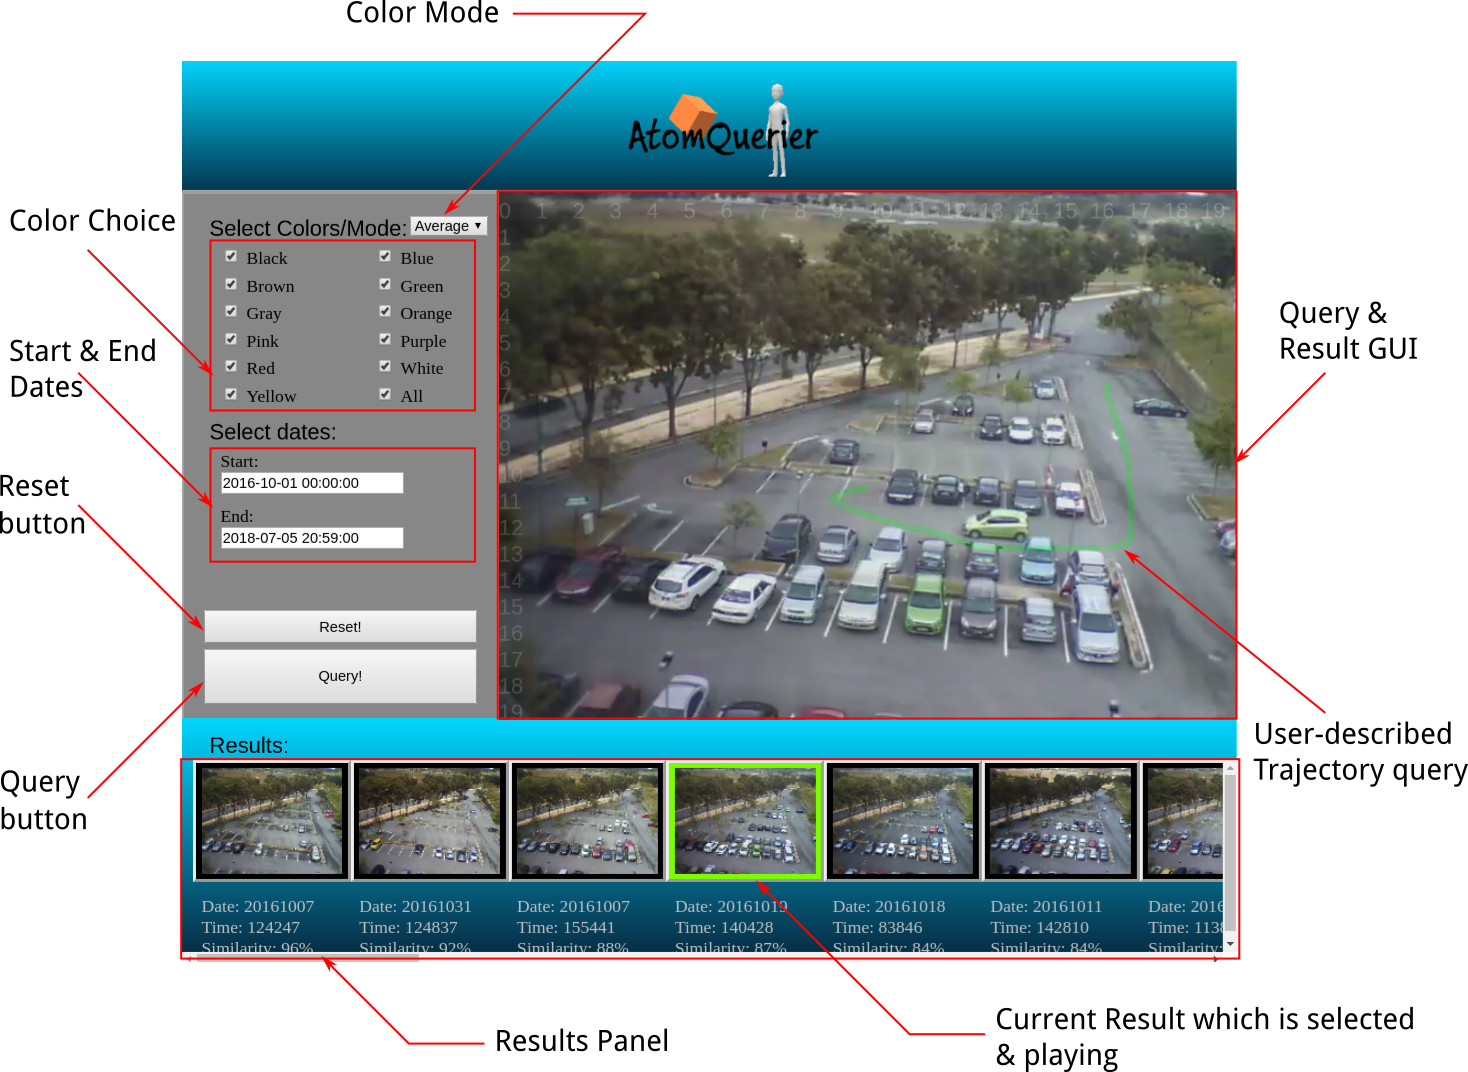
\includegraphics[width=.9\textwidth]{image/retrievalTwo/VISERinterface2.png}
\caption{Search Interface for \versionTwoRet}
\label{fig:versionTwoInterface}
\end{figure}

\subsection{Metrics, Scoring System and Experimental Methodology}

The following subsections describes the scoring system, metrics as well as the evaluation process of the proposed method described in Section \ref{section:versionTwo}. With the main objective of providing users with results that closely resembles the given query, results which are more relevant were sorted such that it would appear higher in the ranked results. In this setting, the performance of the proposed method was measured using the \textit{Precision@K} and normalised Discounted Cumulative Gain (\textit{nDCG}) metrics.

The \textit{Precision@K} metric is used to identify the number of retrieved results which are relevant to the user while the \textit{nDCG} metrics is used to measure how well the retrieval engine's results were sorted for the end users. The idea behind \textit{DCG} metric is that highly relevant results are more useful when it appears higher in rank (hence, higher gain). Users would not need to go through too many results before finding a suitable and relevant result. Likewise, relevant documents which appears lower in the rank should be penalised, hence the discount in its gain.

In order to evaluate the performance of the proposed method, the evaluation of both the trajectory and colour terms were separated. The separation of evaluations allows further understanding on how to improve the retrieval engine as a whole. The evaluation process took on a user study approach.
First, a group of volunteers was introduced to the retrieval engine along with it's features and a sample use case was demonstrated. Next, the volunteers were given full control to draw any query they were interested in. They were then tasked to provide feedback by rating each result with a scale of 1 to 5, with 5 being a result that closely resembles the input query.

The volunteers were given full control of drawing the input query $\mathbb{P}$ to mimic a real world scenario. As there were no limitation on what could be drawn on the search canvas, it was not feasible obtaining the ground truth annotation for each and every possible motion within the one month data time frame. Hence, without these ground truth data, the recall rate could not be measured for this retrieval engine.
While \textit{Precision@K} metrics is commonly used metric in retrieval systems, the main disadvantage of this metric is that the evaluation process is done in a coarse manner. This is because it only provides a binary evaluation of whether or not a particular result is relevant to the query. On the other hand, the \textit{DCG} metric is able to provide a more granular evaluation of the proposed method as the results are evaluated based on its ordered rank along with the relevancy of the result. Figure \ref{fig:dcgGain} illustrates the decreasing gain value of each result as the ranking of the result increases.

\begin{figure}[!ht]
\centering
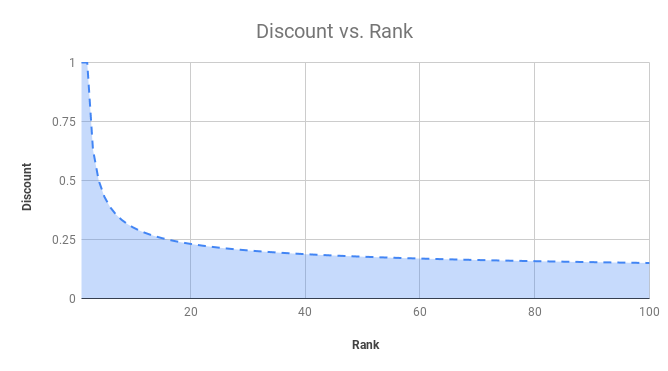
\includegraphics[width=0.9\textwidth]{image/retrievalTwo/discountvsrank.png}
\caption{The Discounted Gain Decreases Exponentially as Rank Increases}
\label{fig:dcgGain}       % Give a unique label
\end{figure}

\begin{equation}
\label{eq:DCGk}
DCG_p = \sum_{p=1}^k\frac{REL_{p}}{\log_2 (\max (p,2))}
\end{equation}

% $DCG@K = \sum_{i=i}^K\frac{REL_{i}}{\log_2 (\max (i,2))}$

Since the Discounted Cumulative Gain metric produces an unbounded value ([0, $\infty$) range), it is not suitable for use when averaging across multiple independent queries. In order to make use of the \textit{DCG} metric, it is converted into the \textit{nDCG} metrics using Equation \ref{eq:nDCG} where the values are now bounded within a [0, 1] range.
\begin{align}
\label{eq:nDCG}
\textit{nDCG}_P = \frac{DCG_P}{IDCG_P}
\end{align}
where:

\hspace{2em} $IDCG_P$ is the ideal DCG score at Rank P in the ideal ranking order.

The following subsections provides in-depth details on the experimental methodology which were designed for the evaluation of the retrieval engine's ability to retrieve both the vehicle trajectory as well as vehicle colours.


\subsubsection{Vehicle Trajectory}
The volunteers were given full control of the user interface and tasked to draw
at least 1 trajectory as an input query. Upon obtaining results from the query,
they were asked to rate each of the resulting trajectory video shot with a scale from 1 to 5, where 1 signifies the least relevant and 5 being the most relevant.

Each query would return at least 25 randomly ordered results. This was done
intentionally to remove any pre-conceived idea of how the results should be
ordered which would affect the way each retrieved results is judged. By removing
the biasness, the volunteers were able to provide a fair and sound evaluation
towards each result, hence, increasing the credibility of the overall results.


\subsubsection{Vehicle colour \& colour Mode}
\label{subsec:vehColor}
As for the evaluation of the vehicle colours, a list of 330 video snippets (30
video snippets for each of the 11 common colours) were presented to the
volunteers. These video snippets were selected using the top 30 results in the
database which contained the highest probability score for each of the 11
colours. The volunteers were then asked to determine the relevance of the colour
term to that particular vehicle for each of the 330 video snippets with the same
scale of 1 to 5.

To further evaluate the performance of the colour semantic extraction process
which was introduced in Section \ref{section:versiontwoColor}, three other
colour modes were included in the evaluation process. These colour modes
represents variations on how the colour terms were extracted using different colour space and distance metrics. These variations are listed in Table \ref{table:ColorVariation}.

\begin{table}[!ht]\centering
\begin{tabular}{|c|l|}
\hline
Colour Mode & Distance Metrics \\
\hline
LUV &
\begin{tabular}{lcl}
\\
$\mean{r}$ &  $=$  & $\frac{C_{1R} + C_{2R}}{2}$\\
$\Delta R$ & $=$ & $C_{1R} - C_{2R}$\\
$\Delta G$ & $=$ & $C_{1G} - C_{2G}$\\
$\Delta B$ & $=$ & $C_{1B} - C_{2B}$\\
\\
$\Delta Colour_{LUV}$ & $=$ &$\sqrt{(2 + \frac{\mean{r}}{256}) \times \Delta R^{2} + 4 \times \Delta G^{2} + (2 + \frac{255 - \mean{r}}{256}) \times \Delta B^{2}}$
\\
\hspace{4em}& & \\
\end{tabular}\\
\hline
HSV &
\begin{tabular}{lcl}
\\
\multicolumn{3}{c}{(As introduced in Section \ref{section:versionOneColorExtract})}
\\

$\Delta{Hue}$ & $=$ & $\min\{ \mid GT_{hue} - Colour_{hue} \mid,  180^{\circ} - \mid GT_{hue} - Colour_{hue} \mid  \}$ \\
$\Delta  Saturation$ & $=$ & $GT_{saturation} - Colour_{saturation}$ \\
$\Delta  Value$ &  $=$ & $GT_{Value} - Colour_{Value}$ \\
\\
$\Delta Colour_{HSV}$ & $=$ & $\sqrt{\Delta{Hue}^{2} + \Delta{Sat}^{2}  + \Delta{Val}^{2} }$
\\
\hspace{4em}& & \\
\end{tabular}\\
\hline
Lab &
\begin{tabular}{lcl}
\\
$\Delta L$ & $=$ & $C_{1L} - C_{2L}$\\
$\Delta a$ & $=$ & $C_{1a} - C_{2a}$\\
$\Delta b$ & $=$ & $C_{1b} - C_{2b}$\\
\\
$\Delta{Colour_{Lab}}$ & $=$ & $\sqrt{\Delta{L}^{2} + \Delta{a}^{2}  + \Delta{b}^{2} }$
\\
\hspace{5em}& & \\
\end{tabular}\\
\hline
Average &
\begin{tabular}{lcl}
\\
$\Delta{Colour_{Average}}$ & $=$ & $\frac{\Delta{Colour_{LUV}} + \Delta{Colour_{HSV}} + \Delta{Colour_{Lab}}}{3}$
\\
\hspace{4em}& & \\
\end{tabular}\\
\hline
\end{tabular}
\caption{Variation of Colour Distance Metrics Used}
\label{table:ColorVariation}
\end{table}


\subsection{Results and Analysis}

The results for both components (Vehicle Trajectory \& Vehicle Colour) are
recorded in this section. As the results were evaluated using a scale from 1 to
5, these results were first converted into a binary evaluation (True(1) /
False(0)) for the \textit{Precision@K} evaluation metrics. Here, results scoring with an average of 3 and above are considered relevant to the query. Each relevant (True(1)) result \textit{(n)} will then contribute to the \textit{Precision@K} score (see Equation \ref{eq:p@k}).
 \begin{equation}
\label{eq:p@k}
Precision@K =  \frac{\sum_{n=1}^K \begin{cases}1 \rightarrow True, & AvgScore(Result_n)\geq 3\\0 \rightarrow False, & AvgScore(Result_n)< 3 \end{cases}} {K}
\end{equation}

\subsubsection{Vehicle Trajectory}
A total of eleven restriction-free trajectories were drawn by six volunteers.
The volunteers were allowed to draw any kind of desired trajectory on the input
canvas.
Figure \ref{fig:versionTwoTrajquery} shows a compilation of these trajectories
overlaid over the car park scene, these trajectories covered a majority of the
scene while showing a good mixture of different queries.
Even though some of the queries exceeded the tracking area of the tracker,
the retrieval engine still managed to retrieved results which has the closest
resemblance to the given queries. As previously mentioned, the performance of
the retrieval engine was measured using \textit{Precision@K} along with the
\textit{normalised Discounted Cumulative Gain} (\textit{nDCG}) metrics.

\begin{figure}[!t]
  \centering
    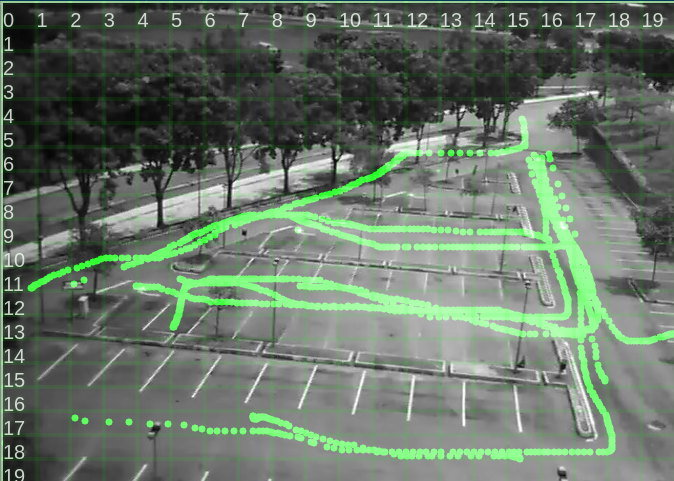
\includegraphics[width=0.8\linewidth]{image/retrievalTwo/trajquery.png}
  \caption{Compilation of Trajectory Queries Provided by Volunteers}
  \label{fig:versionTwoTrajquery}
\end{figure}

Even though the errors from the tracker\cite{lim2017} cascaded into database,
results due to tracker error was not removed to provide a broad idea of the
retrieval engine's performance when working with trackers which are currently
available. First, the \textit{Precision@K} of the retrieval engine was measured
and recorded, Figure \ref{fig:versionTwoPreAtK} contains the plot of the
average \textit{Precision@K} result. The result shows that the retrieval engine
managed to retrieve video shots which were relatively relevant to the user's
query with an average precision of 76\% with a steady decline in its precision
as the K (number of results) increases. This was an expected outcome as it is
common occurance in a regular retrieval engine.

\begin{figure}[!ht]
  \centering
    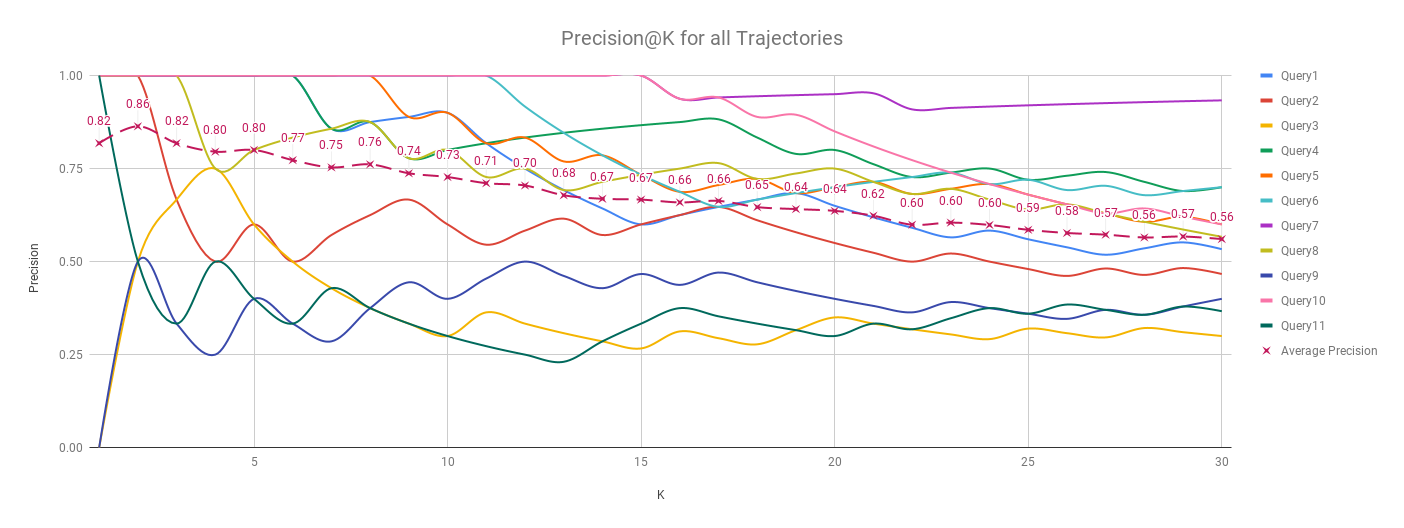
\includegraphics[width=\linewidth]{image/retrievalTwo/p@k.png}
  \caption{Precision at K for All Trajectory Queries}
  \label{fig:versionTwoPreAtK}
\end{figure}

Next, in order to determine the retrieval engine's overall performance in
regards to how the results were ordered, the average \textit{nDCG} score for
all eleven trajectory queries were measured and plotted in Figure
\ref{fig:ndcgWithError}. As a whole, the average \textit{nDCG} score lies along
the 83\% region, which means that the results ordered in the best possible
manner 83\% of the time.
In an ideal scenario, the scores should remain at 1, signifying that the
results were ordered perfectly. However, in this experiment, the \textit{nDCG}
score shows an increase as the number of retrieved results were evaluated.
While this is not desirable, this behaviour was expected in a non-ideal
condition.

\begin{figure}[!ht]
  \centering
    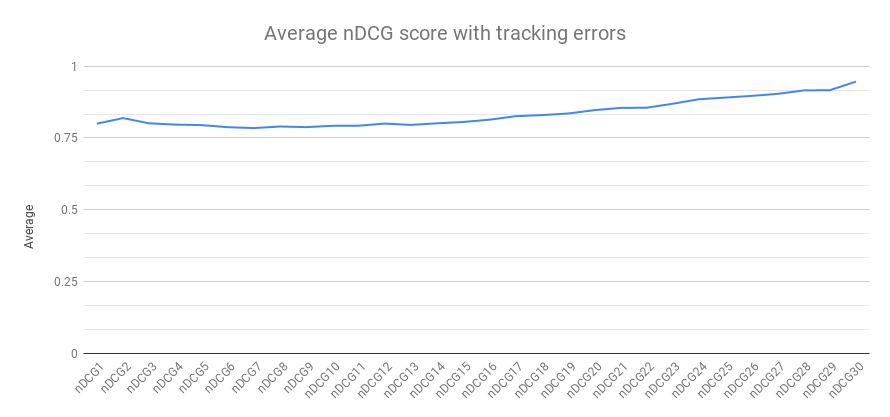
\includegraphics[width=0.9\linewidth]{image/retrievalTwo/averageNDCG.png}
  \caption{Average Normalised Discounted Cumulative Gain Score}
  \label{fig:ndcgWithError}
\end{figure}

To further break down the evaluation process of the retrieval engine's
performance, as per the previous retrieval model's evaluation, the trajectory
queries were also divided into two categories: \textit{simple} and
\textit{complex} trajectories. \textit{Simple} trajectories refers to
trajectories that moves in a single direction without any turning (such as a
straight line) while \textit{complex} trajectories refers to movements which
consist of more than one simple motion.
Table \ref{table:versionTwoComplexSimple} shows the category of each query while
the \textit{Precision@K} results are plotted in Figure
\ref{fig:versionTwoPatKAll}.

For simple trajectories, the Precision@K scores a high 100\% at the beginning
and slowly decrease to around 68\% as the number of retrieved results (K) were
reviewed. All the simple queries shows rather consistent results which are as
expected. As for complex trajectories, the precision at k=1 started at 67\% and
dropped further to 46\% at the end of 30 results. Even though Query 1 and Query
6 belongs in the complex trajectory category, the first 10 results shows rather
high precision. However, the majority of the other complex trajectory did not
perform as well as Query 1 and Query 6. The overall Precision@K results shows
an expected behaviour where the precision would be high in the early K region,
and would slowly decrease as K increases.

% Please add the following required packages to your document preamble:
% \usepackage{multirow}
\begin{table}[!ht] \centering
\begin{tabular}{|c|c|c|}
\hline
\multicolumn{1}{|c|}{\textbf{Trajectory Category}} & \textbf{Query Number} & \textbf{Minimap}\\ \hline
\multirow{5}{*}{Simple} & Query 4 & 
\includegraphics{image/minimaps/query_04.png} \\ \cline{2-3}
 & Query 5 & 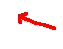
\includegraphics{image/minimaps/query_05.png} \\ \cline{2-3}
 & Query 7 & 
\includegraphics{image/minimaps/query_07.png} \\ \cline{2-3}
 & Query 8 & 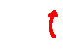
\includegraphics{image/minimaps/query_08.png} \\ \cline{2-3}
 & Query 10 & 
\includegraphics{image/minimaps/query_10.png} \\ \hline
\multirow{6}{*}{Complex} & Query 1 & 
\includegraphics{image/minimaps/query_01.png} \\ \cline{2-3}
 & Query 2 & 
\includegraphics{image/minimaps/query_02.png} \\ \cline{2-3}
 & Query 3 & 
\includegraphics{image/minimaps/query_03.png} \\ \cline{2-3}
 & Query 6 & 
\includegraphics{image/minimaps/query_06.png} \\ \cline{2-3}
 & Query 9 & 
\includegraphics{image/minimaps/query_09.png} \\ \cline{2-3}
 & Query 11 & 
\includegraphics{image/minimaps/query_11.png} \\ \hline
\end{tabular}
\caption{Queries and the Corresponding Trajectory Type}
\label{table:versionTwoComplexSimple}
\end{table}

As a whole, both \textit{simple} and \textit{complex} queries shows reasonably
good performance in terms of its precision, however, when evaluated
individually, the \textit{complex} queries shows poorer results. Next, the
\textit{nDCG} score of both the \textit{simple} and \textit{complex} trajectory
queries were evaluated and plotted in Figure \ref{fig:versionTwoNDCG}(a) and
Figure \ref{fig:versionTwoNDCG}(b) respectively. Contrary to coarse results
obtained using \textit{Precision@K}, the \textit{nDCG} score is able to provide
an indepth evaluation as it takes the relevancy into consideration.


\begin{figure}[htb!]
  \centering
\begin{tabular}{c}
 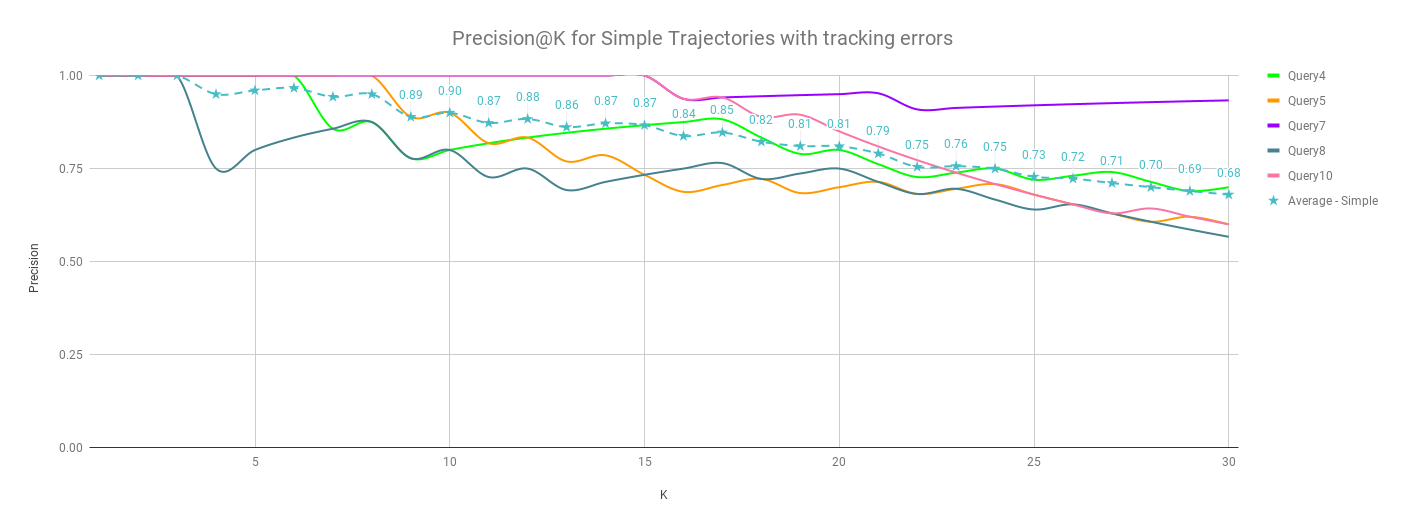
\includegraphics[width=0.9\linewidth]{image/retrievalTwo/p@k_simple.png}\\
 (a) \textit{Precision@K} for Simple Trajectories \\
 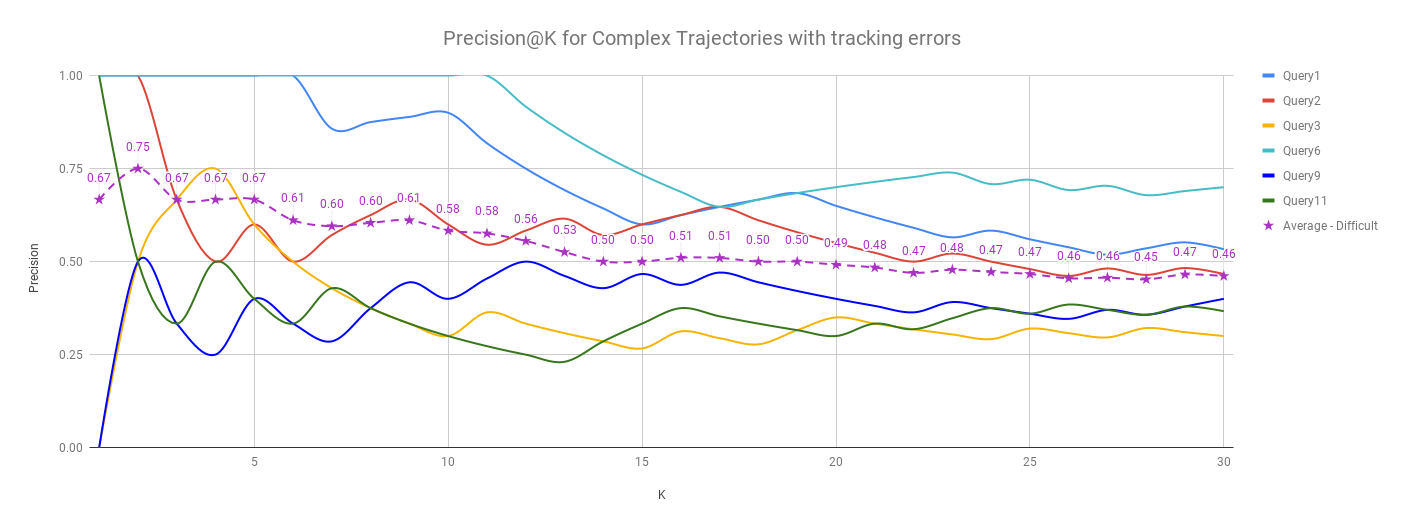
\includegraphics[width=0.9\linewidth]{image/retrievalTwo/p@k_complex.png} \\
 (b) \textit{Precision@K} for Complex Trajectories
\end{tabular}
\caption{\textit{Precision@K} for Simple and Complex Trajectories Queries}
\label{fig:versionTwoPatKAll}
\end{figure}


\begin{figure}[htb!]
  \centering
  \begin{tabular}{c}
   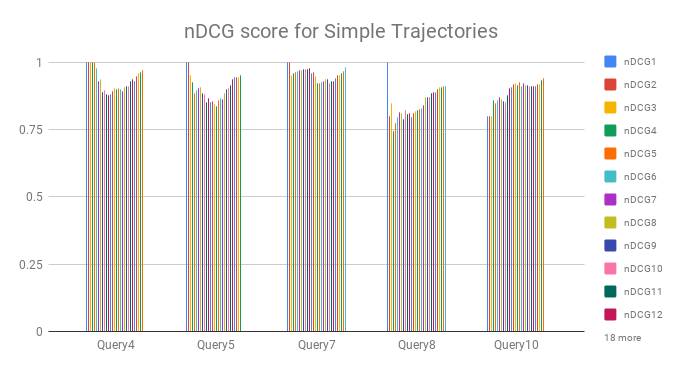
\includegraphics[width=0.9\linewidth]{image/retrievalTwo/ndcgSimple.png}\\
   (a) \textit{nDCG} for Simple Trajectories \\
   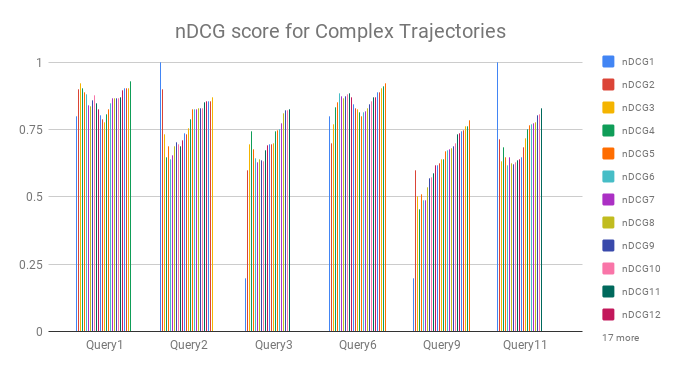
\includegraphics[width=0.9\linewidth]{image/retrievalTwo/ndcgComplex.png} \\
   (b) \textit{nDCG} for Complex Trajectories
  \end{tabular}
  \caption{Normalised Discounted Cumulative Gain for Simple and Complex
  Trajectories Queries}
  \label{fig:versionTwoNDCG}
\end{figure}

Based on the graph, the difference between the simple and complex trajectories
are rather distinct. The overall nDCG score for the queries of simple
trajectories howers high around the 91\% region while the nDCG score for complex
trajectories were in the neighbourhood of 75\%. The results here shows that the
retrieval engine had an easier time sorting simple trajectories in the best
ranking order while having some difficulty organising the complex trajectories
using the $D_{chamfer}$ metrics.

Additional comparison between Chamfer Distance and various other distance
measures were also computed to further understand the difference, advantages
and properties of these methods. Table \ref{table:DistanceCompare} contains a
compilation of 7 different test cases compared against a single sample ground
truth data. These test cases were then tested using 5 different distance
measures: Chamfer Distance, Dynamic Time Warping, Hausdorff Distance, Earth
Mover Distance, and Euclidean Distance. In all cases, smaller numbers
represents lower distance (higher similarity) while larger numbers represents
larger distance (lower similarity).

As a baseline comparison, a simplistic approach using Euclidean Distance was
also measured. The results obtained from Euclidean Distance shows minimal
difference in the raw results when comparing the best case and worst test case.
While the normalised results shows better results, the normalised result is not
a useful metrics as it only represents the distribution in the 7 test cases. In
an actual retrieval process, we are not able to obtain these score during
runtime. Based on the results in Table \ref{table:DistanceCompare}, it is
noticed that Earth Mover Distance favours similar shapes as it is able to
effectively deal with scaling of shapes. While useful in other applications,
this is not a desirable property in the context of a retrieval engine in a car
park setting. As expected, this distance measure heavily penalises Test 1, which
contains a mirrored shape.

In the case of Hausdorff distance, it is noticed that this distance measure
often measures the maximum distance of a set to the nearest point in the other
set which is usually used for image matching. It is also observed that this
distance measure was not able to handle Test 2 which deals with directional
inputs, this shows that this metric was not a suitable candidate in our
retrieval engine. The overall results shows that both Chamfer Distance and
Dynamic Time Warping were candidate methods  as they have relatively good and
similar performance in those 7 test cases. However, Chamfer Distance was able
to return higher difference ratio between the best case and worst case test
case. This attribute is extremely desireable and very useful when sorting huge
numbers of trajectories from the database.

Even though the overall results using Chamfer Distance were relatively good,
the implementation of this distance metrics in the proposed method is not
without its faults. Observation of the results shows that Chamfer Distance
performs poorly when (i) a trajectory is compared against a much shorter
trajectory that intersects at a particular point or (ii) two trajectories
of similar shape turning into 2 different junctions. In both examples,
the obtained $D_{chamfer}$ were relatively low, hence these results could
potentially be retrieved, these examples can be found in Figure
\ref{fig:chamferDisadvantage}.

\begin{figure}[htb!]
  \centering
\begin{tabular}{cc }
 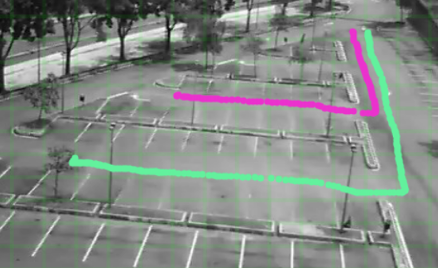
\includegraphics[width=0.45\linewidth]{image/retrievalTwo/chamferDisadv2.png} &
 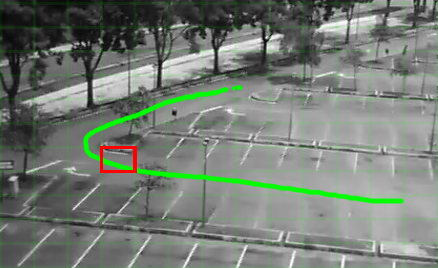
\includegraphics[width=0.45\linewidth]{image/retrievalTwo/chamferDisadv1.png} \\
 (a) Two trajectories with similar shape &
 (b) Trajectory intersecting with a point \\
\end{tabular}
\caption{Disadvantages of Chamfer Distance} \label{fig:chamferDisadvantage}
\end{figure}


% Please add the following required packages to your document preamble:
% \usepackage{graphicx}
% \usepackage{lscape}
\begin{landscape}

\begin{table}[]
\resizebox{23cm}{!}{%
\centering
\begin{tabular}{|l||l|l|l|l|l|l|l|}
\hline
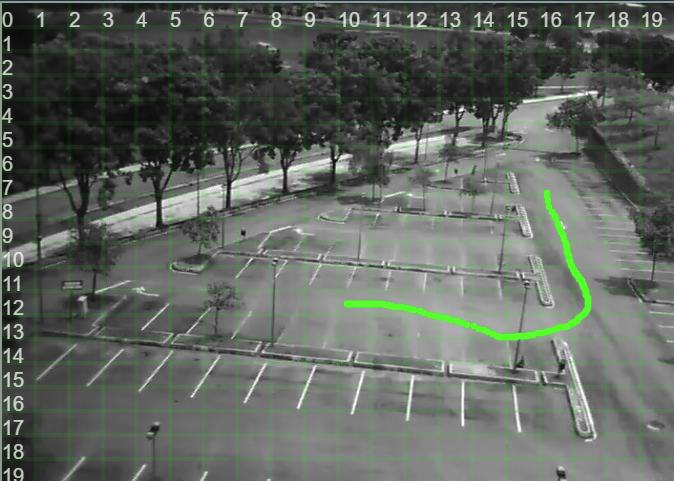
\includegraphics[scale=0.25]{image/suppResults/gt.PNG}
 & 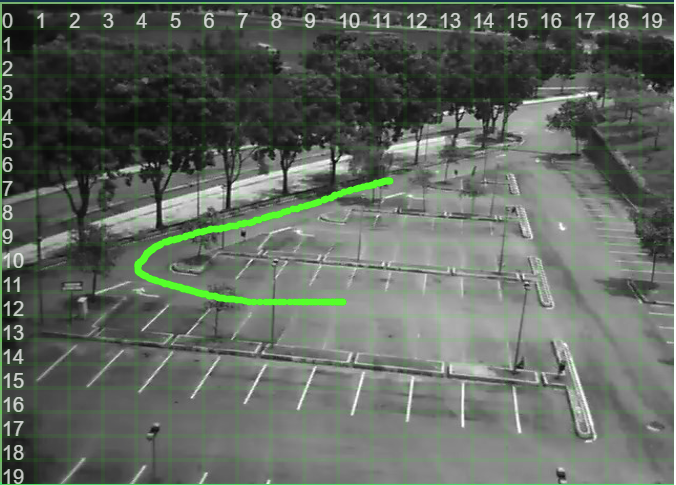
\includegraphics[scale=0.25]{image/suppResults/q1.PNG}
 & 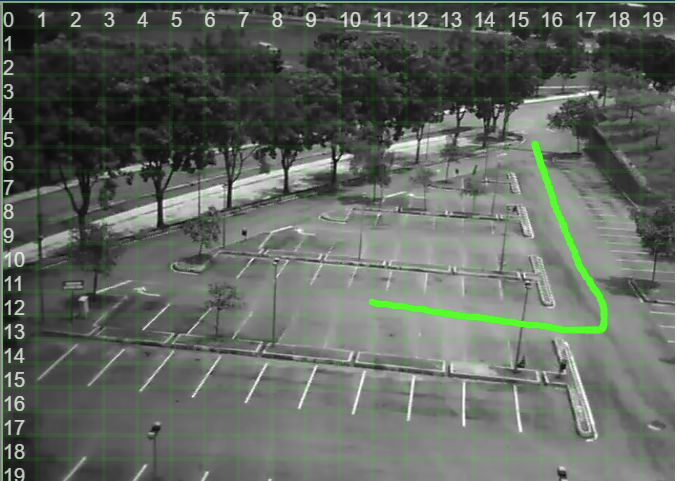
\includegraphics[scale=0.25]{image/suppResults/q2.PNG}
 & 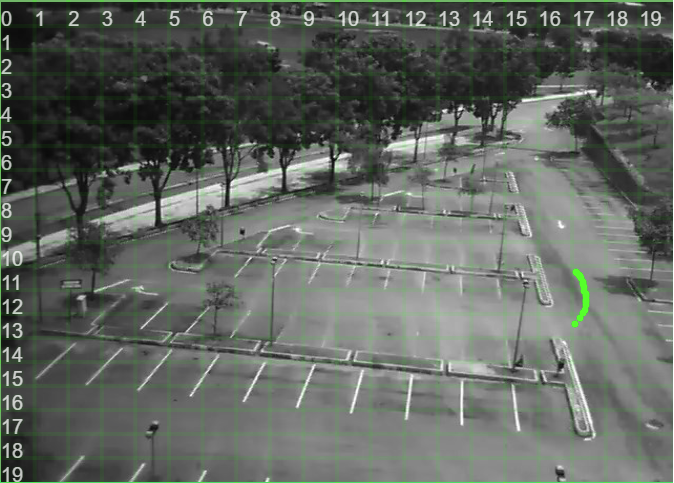
\includegraphics[scale=0.25]{image/suppResults/q3.PNG}
 & 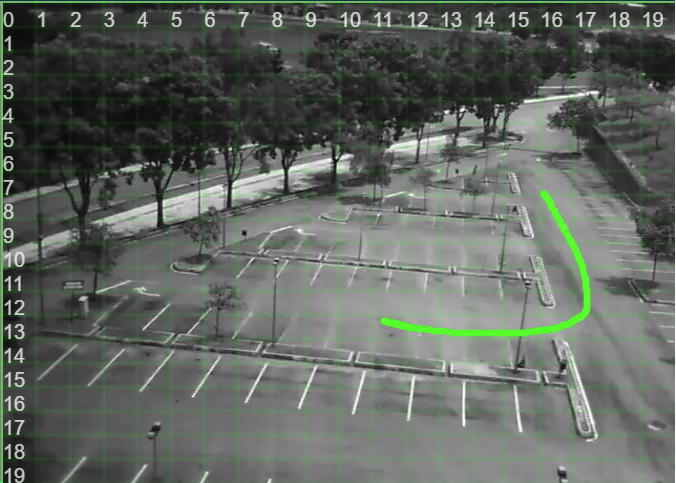
\includegraphics[scale=0.25]{image/suppResults/q4.PNG}
 & 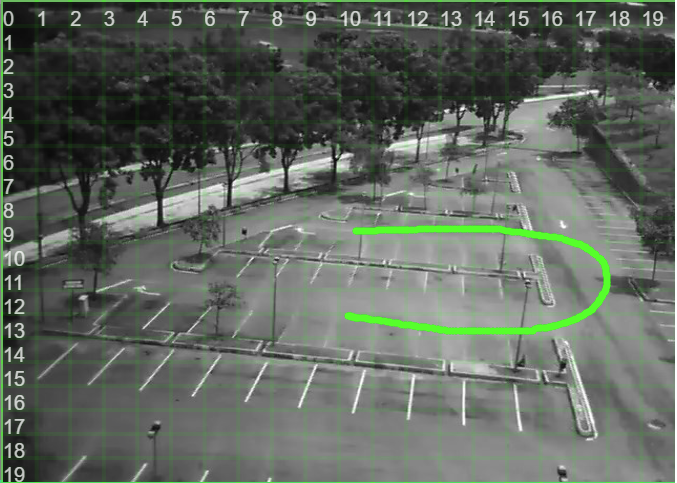
\includegraphics[scale=0.25]{image/suppResults/q5.PNG}
 & 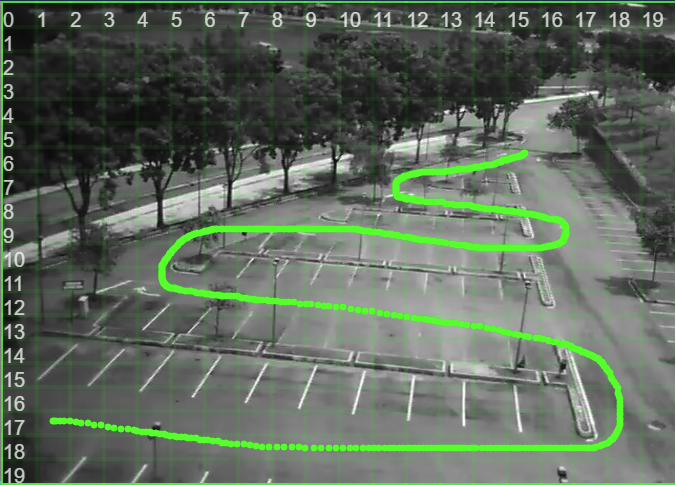
\includegraphics[scale=0.25]{image/suppResults/q6.PNG}
 & 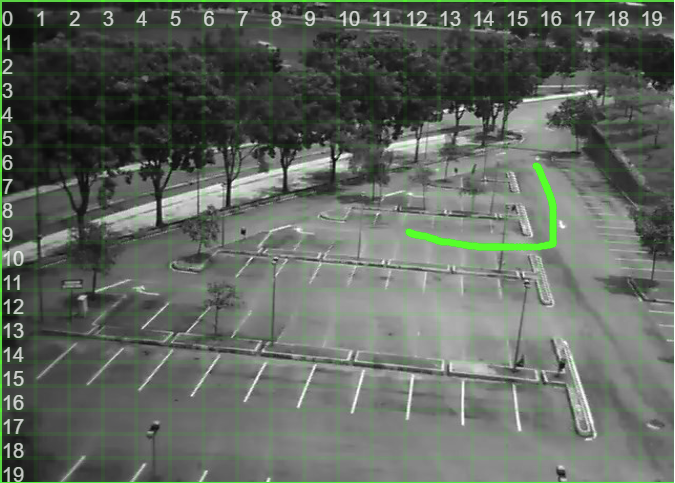
\includegraphics[scale=0.25]{image/suppResults/q7.PNG} \\ \hline
GT Sample & \begin{tabular}[r]{@{}l@{}}Test 1:\\ Mirror\end{tabular} & \begin{tabular}[r]{@{}l@{}}Test 2:\\ Opposite Direction\end{tabular} & \begin{tabular}[r]{@{}l@{}}Test 3:\\ Short Trajectory\end{tabular} & \begin{tabular}[r]{@{}l@{}}Test 4:\\ Highly Resemble GT\end{tabular} & \begin{tabular}[r]{@{}l@{}}Test 5:\\ Partially Resemble GT\end{tabular} & \begin{tabular}[r]{@{}l@{}}Test 6:\\ Long Trajectories\end{tabular} & \begin{tabular}[r]{@{}l@{}}Test 7:\\ Similar Shape\end{tabular} \\ \hline
\textbf{Chamfer Distance} & 0.02565 (1503.21) & 0.0169 (987.84) & 0.0246 (1444.00) & 0.0001 (6.25) & 0.0060 (353.89) & 0.9205 (53937.33) & 0.0062 (361.00) \\ \hline
\textbf{Dynamic Time Warping} & 0.0503 (176.97) & 0.0344 (121.08) & 0.0604 (212.31) & 0.0033 (11.62) & 0.0239 (83.99) & 0.8079 (2841.17) & 0.0198 (69.57) \\ \hline
\textbf{Hausdorff Distance} & 0.2042 (7.07) & 0.0647 (2.24) & 0.2021 (7.00) & 0.0407 (1.41) & 0.0866 (3.00) & 0.2974 (10.30) & 0.1042 (3.61) \\ \hline
\textbf{Earth Mover Distance} & 0.4112 (0.96) & 0.0942 (0.22) & 0.0342 (0.08) & 0.0021 (0.01) & 0.3127 (0.73) & 0.1456 (0.34) & 0.0000 (0.00) \\ \hline
\textbf{Euclidean Distance} & 0.1171 (5.00) & 0.1656 (7.07) & 0.1424 (6.08) & 0.0703 (3.00) & 0.0661 (2.82) & 0.3645 (15.56) & 0.0740 (3.16) \\ \hline
\end{tabular}%
}
\caption{Comparison of Difference Distance Measures against 7 Different Test
  Scenarios Against a Ground Truth Sample Data. The results are represented by
  Normalised Results Followed by the Actual Distance Measure obtained in
  Brackets. Smaller Numbers are Represents Closer Similarity. Euclidean Distance
  acted as a simplistic approach towards this problem, and was used as a
  baseline comparison. The results shows that Earth Mover Distance favoured
  cases where the shapes were similar (Test 7) and penalised a mirrored shape
  (Test 1). Hausdorff distance failed to provide good dissimilarity score for
  Test 2 which was used to test the ability to differentiate directions.
  Overall, Chamfer Distance and Dynamic Time Warping method was able to provide
  comparable results, however, Chamfer Distance came up top as it is able to
  provide a larger margin between the best and worst test cases. This property
  is desireable when comparing huge numbers of trajectories.}
\label{table:DistanceCompare}

\end{table}
\end{landscape}


However, as a whole, despite the flaws of Chamfer Distance, the implementation
of $D_{chamfer}$ in the retrieval engine provided relatively good results
(Average \textit{Precision@K} = 76\%) that were sorted in an organised and
useful manner (\textit{nDCG} score = 83\%). In my opinion, the use of Chamfer
Distance can be extended to other datasets of similar properties for the
retrieval purposes.

\subsubsection{Vehicle Colour \& Colour Mode}
\label{subsec:vehiclecolourchamferdistanceexperiment}

As mentioned in Section \ref{subsec:vehColor}, a total of 330 video snippets
were extracted from the top 30 results of each colour modes.  As four colour
modes were tested, the six volunteer were split into groups of three and were
given two sets of data to evaluate. The results of the average
\textit{Precision@K} metric for each of the colour modes were tabulated in
Figure \ref{fig:colorspace_score} while Table \ref{tab:avg@k} provides a high
level overview of the results across K = 1 to 30. Similar to the evaluation
process of the vehicle trajectories, this time, the volunteers were asked to
determine the relevance of the colour term to that particular vehicle for each
of the video snippets with a scale of 1 to 5.

\begin{table}[!t]
	\centering
	\caption{Average Precision @ K for Each Colour Metrics}
	\label{tab:avg@k}
\begin{tabular}{c||c|c|c|c|c|c|c|c|c|c}
K & 1 & 2 & 3 & 4 & 5 & 10 & 15 & 20 & 25 & 30  \\ \hline \hline
\rowcolor{yellow} LUV  & 0.91 & 0.91 & 0.91 & 0.86 & 0.85 & 0.69 & 0.62 & 0.60 & 0.63 & 0.60 \\
Lab  & 0.27 & 0.27 & 0.27 & 0.25 & 0.24 & 0.24 & 0.24 & 0.23 & 0.22 & 0.22 \\
HSV & 0.27 & 0.36 & 0.30 & 0.27 & 0.29 & 0.25 & 0.25 & 0.23 & 0.21 & 0.21 \\
Avg & 0.09 & 0.18 & 0.15 & 0.16 & 0.16 & 0.18 & 0.18 & 0.20 & 0.23 & 0.23 \\
\end{tabular}
\end{table}


\begin{figure}[htb!]
  \centering
\begin{tabular}{cc}
 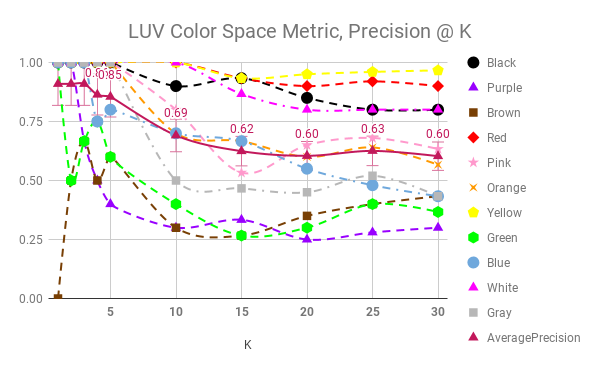
\includegraphics[width=0.5\linewidth]{image/new/luv@k.png} &
 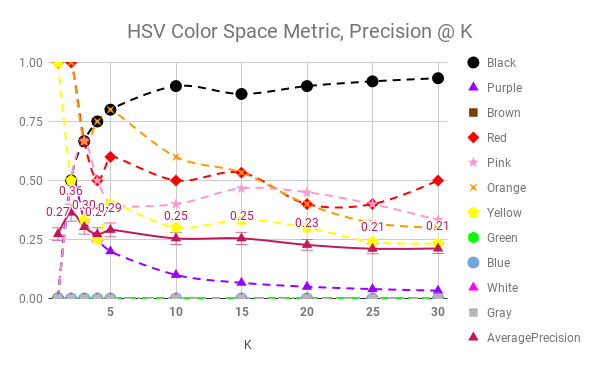
\includegraphics[width=0.5\linewidth]{image/new/hsv@k.png}\\
 (a) LUV colour Mode &
 (b) HSV colour Mode \\
 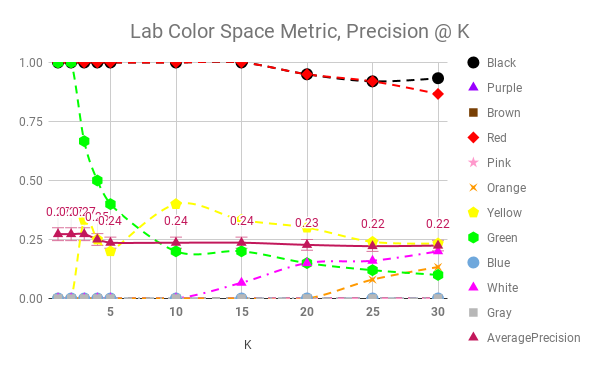
\includegraphics[width=0.5\linewidth]{image/new/lab@k.png} &
 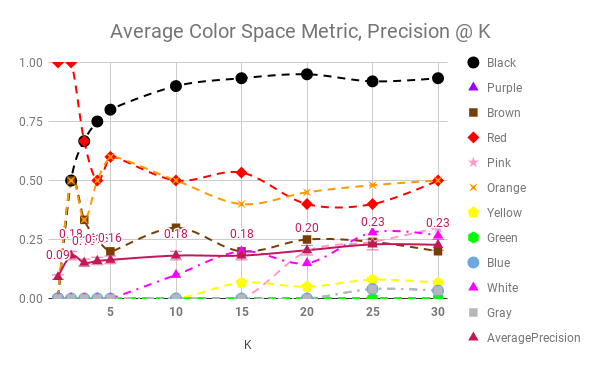
\includegraphics[width=0.5\linewidth]{image/new/avg@k.png} \\
 (c) Lab colour Mode&
 (d) Average colour Mode \\
\end{tabular}
\caption{\textit{Precision@K} for Each colour Mode} \label{fig:colorspace_score}
\end{figure}

The \textit{Precision@K} results of the LUV colour mode showed the best results
among the other colour modes used to extract the colour term. The average
precision at K=1 is recorded at 91\%, however, by the time K=10, the precision
has dropped to an average precision of 69\% and gradually drops to 60\% when K
reached 30. The colours Yellow, Red, Black, and White showed consistent results
throughout the experiment while colours like Purple, Green and Brown fared
poorly. This was likely because there were not many cars which were highly
saturated in those shades of colours.

When comparing with the other colour modes, Black colour provided relatively
consistent results throughout the entire experiment. The average precision for
the HSV and Lab colour modes staggered around the 25\% region. It is also
observed that the retrieval of Red and Black colour vehicles perform
significantly better in the Lab colour space when compared to the other colours,
the average precision of these two colours are in the 90\% vicinity.

During the preparation phase of the experimental methodology, the average
colour mode was designed with the goal of maximising the strength of each
colour modes while averaging out the weaknesses. However, based on the
conducted experiment, it was surprising to see the underwhelming performance of
the HSV and Lab colour mode. Hence, the average colour mode also took a dive in
terms of the precision. However, this colour mode did live up to its expectation
in maximising the strengths of each colour modes. Based on the results
tabulated, the precision when retrieving Black colour vehicles was well except
for the initial precision during the early K region which were unexpected.

To further analyse the performance of the colour modes used, the confusion
matrix of each colour mode used is plotted in Figure
\ref{fig:colorspace_Confuscore} using 30 results for each colour term (with a
total of 330 results for each colour space). The X-axis represents the Actual
Colour, while the Y-axis represents the Predicted Colour. The colours in the
confusion matrix were arranged in the following order: Black, Purple, Brown,
Red, Pink, Orange, Yellow, Green, Blue, White, Gray. This colours were ordered
based on its perceived similarity in terms of saturation and brightness.
In the figure, the X-axis also contains an additional row which indicates
numbers of results which were due to tracking error in the initial tracking
phase.

\begin{figure}[htb!]
  \centering
  \begin{tabular}{cc}
    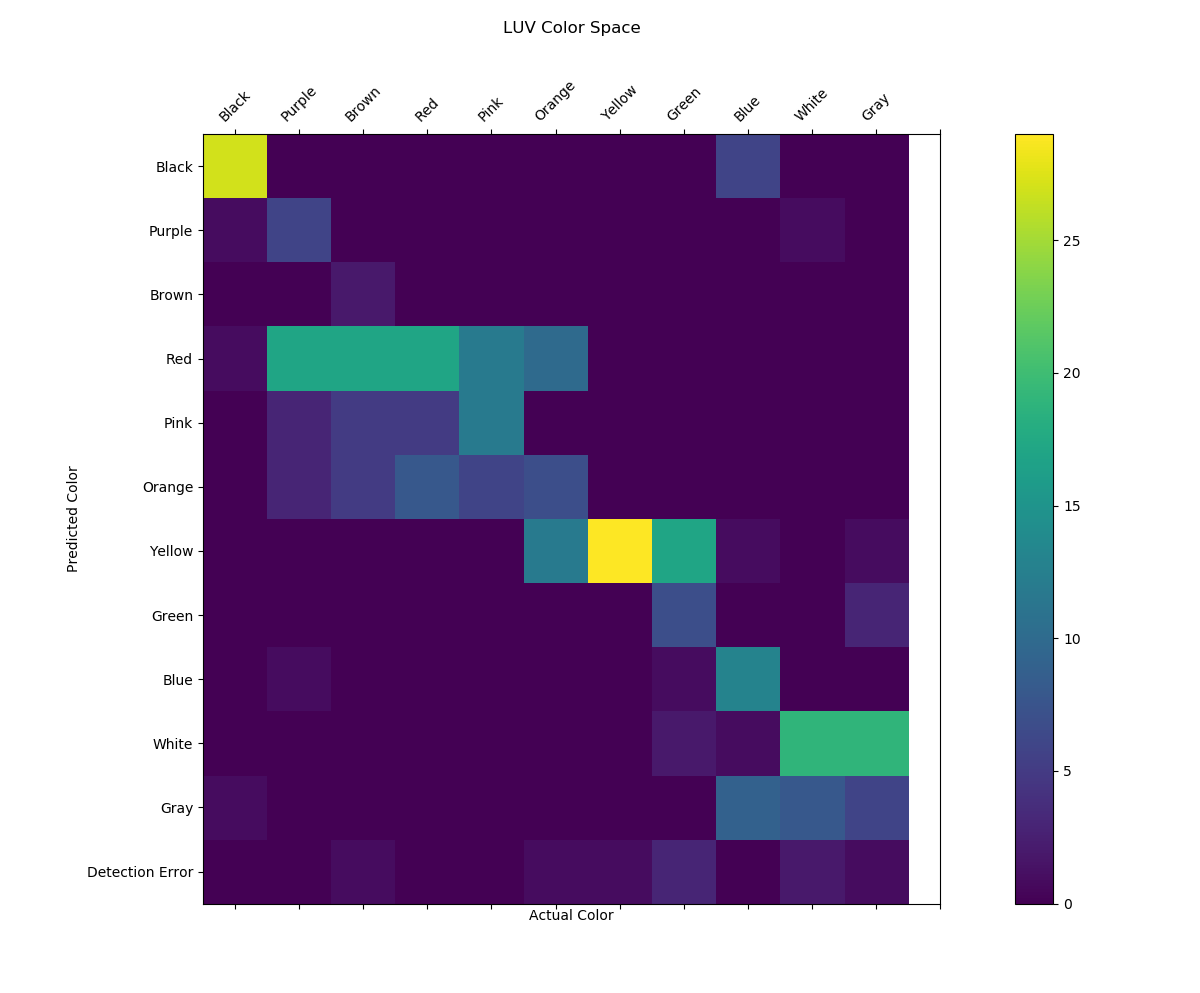
\includegraphics[width=0.4\linewidth]{image/retrievalTwo/luvCM.png} &
    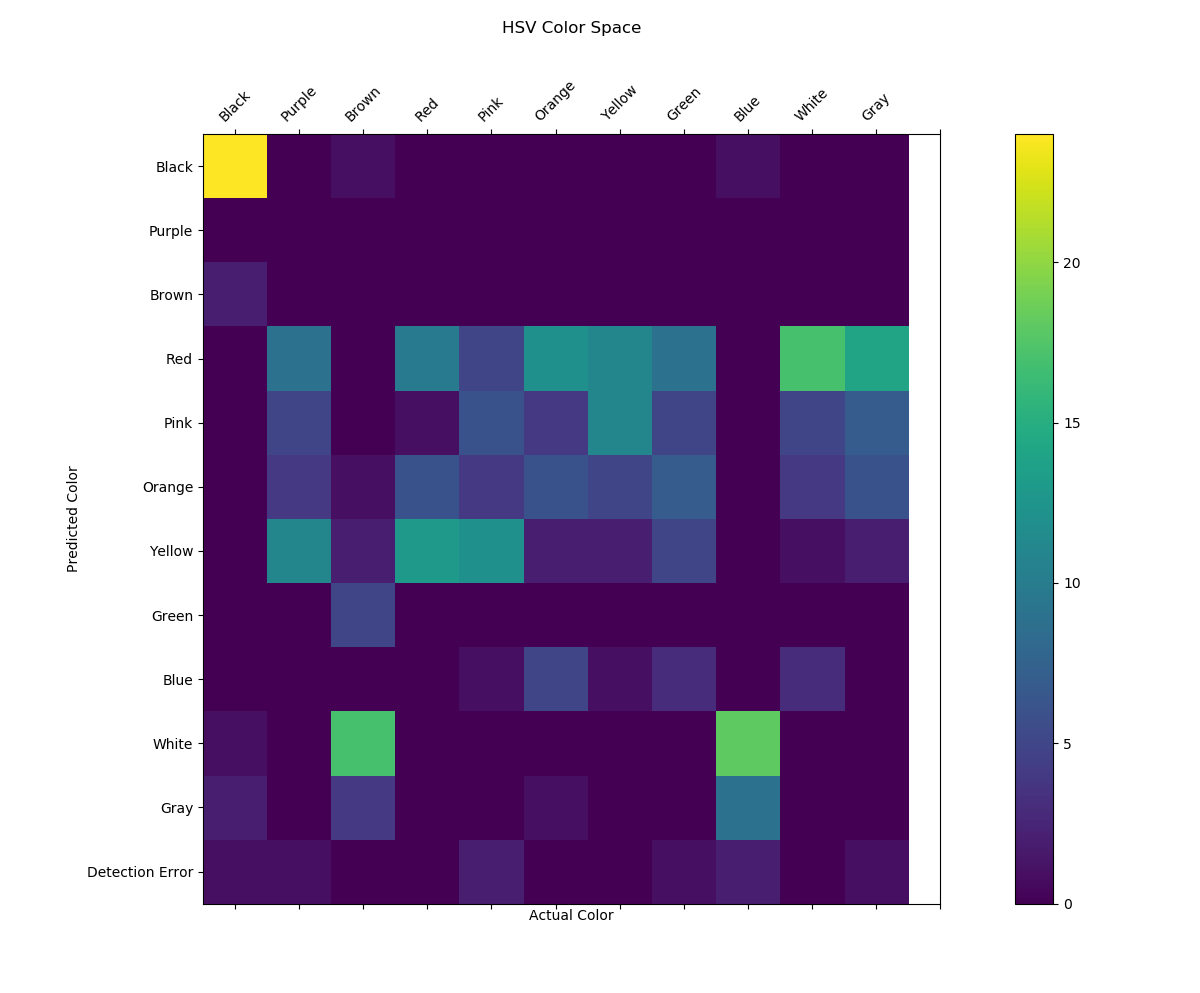
\includegraphics[width=0.4\linewidth]{image/retrievalTwo/hsvCM.png} \\
    (a) LUV colour Mode & (b) HSV colour Mode \\
    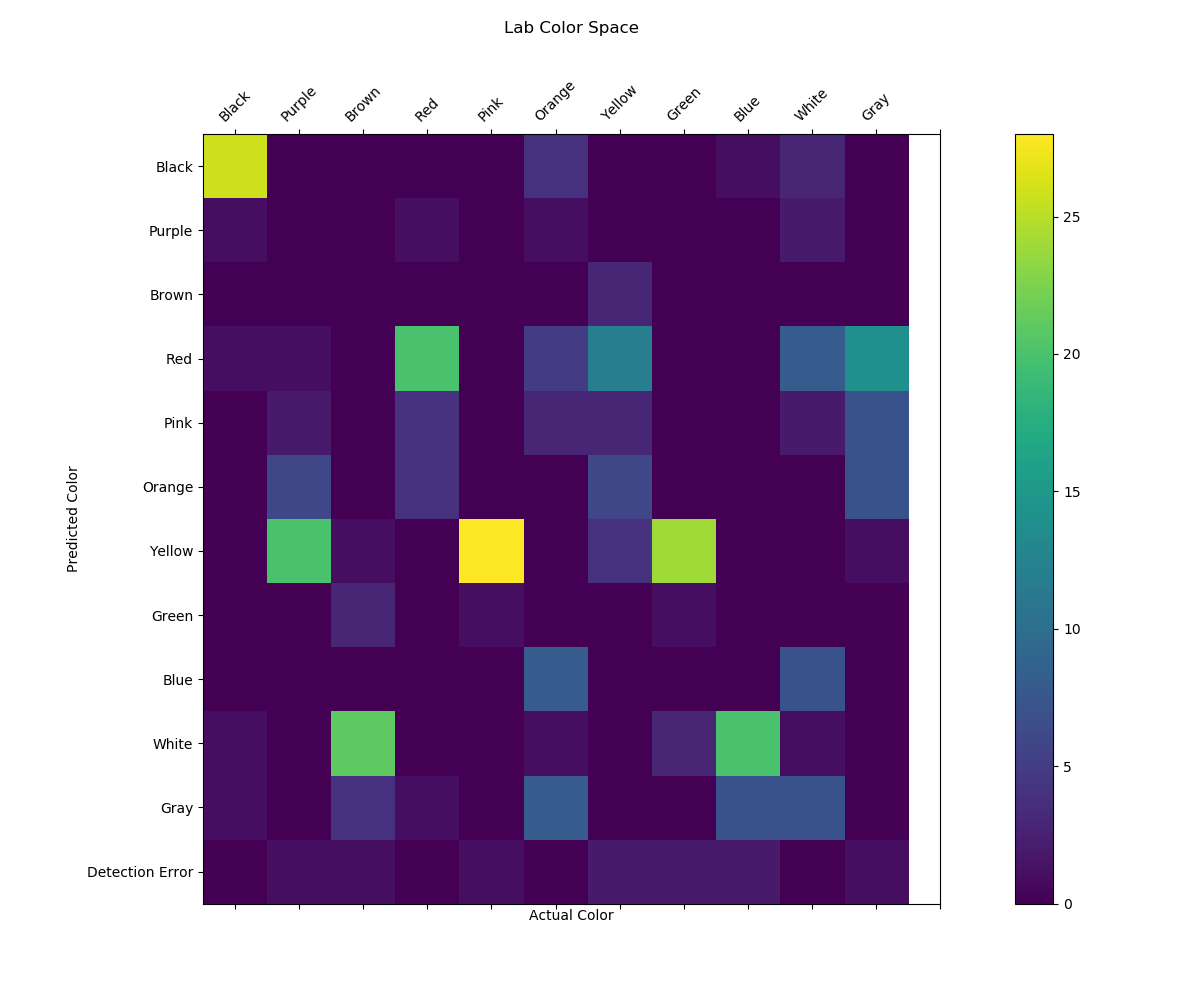
\includegraphics[width=0.4\linewidth]{image/retrievalTwo/labCM.png} &
    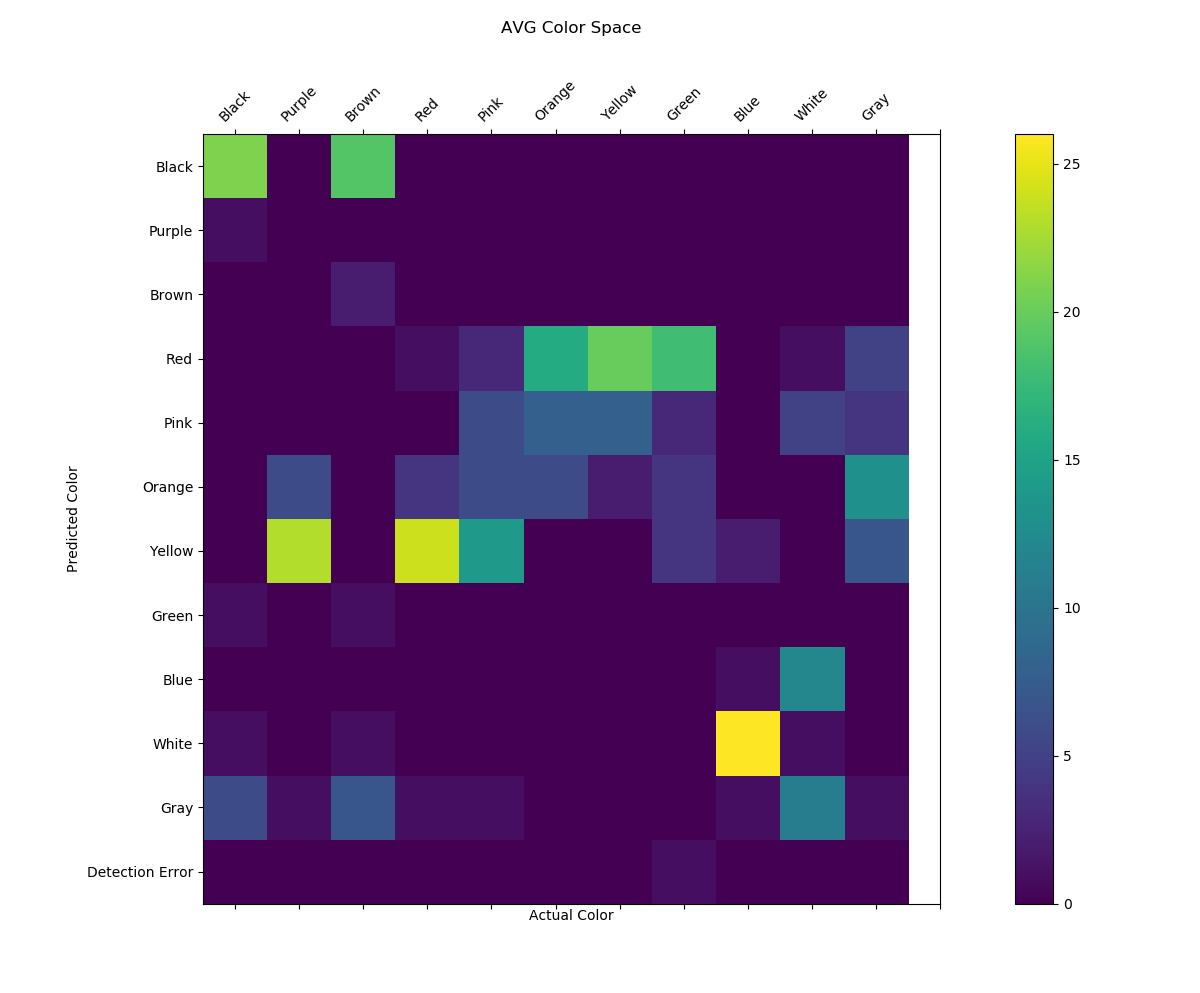
\includegraphics[width=0.4\linewidth]{image/retrievalTwo/avgCM.png} \\
    (c) Lab colour Mode & (d) Average colour Mode \\
  \end{tabular}
  \caption{Comparison Between the colour Modes Using Confusion Matrix}
  \label{fig:colorspace_Confuscore}
\end{figure}

Upon further inspection of the tabulated confusion matrices, the results shows
similar output when compared with the \textit{Precision@K} results recorded
from the volunteers via the scoring method. Both the results tallies in their
finding that the low cost LUV colour mode proposed by Riemersma\cite{riemersma}
outperforms the other colour modes. The Euclidean distance metrics used in the
HSV colour mode to extract the colour terms performed the worst with not much
variation in the results for each colour. On the other hand, the Lab colour
mode's results showed a considered amount of accuracy for strongly distinct
colours such as Red and Black but fails to differentiate the rest as visualised
in Figure \ref{fig:colorspace_Confuscore}(C).

Given that the LUV colour mode's \textit{Precision@K} metrics outperformed the
rest with a precision of 85\% at k=5, while the other colour modes barely
reached the 30\% mark, only the normalised Discounted Cumulative Gain
(\textit{nDCG}) for the LUV colour mode results were measured and plotted to
understand the performance of the retrieval engine in terms of how well the
results were sorted. The \textit{nDCG} metrics was not measure for the HSV, Lab
and Average colour space metrics as they did not perform well, hence, the order
of the results does not represent the actual performance of the retrieval
engine. The Discounted Cumulative Gain result was also visualised in
Figure \ref{fig:colorndcg}.

The Bar chart is used to represent the number of results the user has to view
in order to find a relevant document, hence a chart where the results
consistently stays at the high 80-100\% area shows that the ranking of the
results were done in one of the best ways possible. The Radar chart on the
other hand, represents the overall performance of a particular colour over the
number of results the user has to view in order to find a relevant document.
Both of the charts clearly visualise that most colours were retrieved
accurately and sorted in the a relatively good order with an astounding
performance of high 80-90\% except for Brown and Green colour where the
performance only reach the best at the end of 30 results.


\begin{figure}[htb!]
  \centering
  \begin{tabular}{c}
    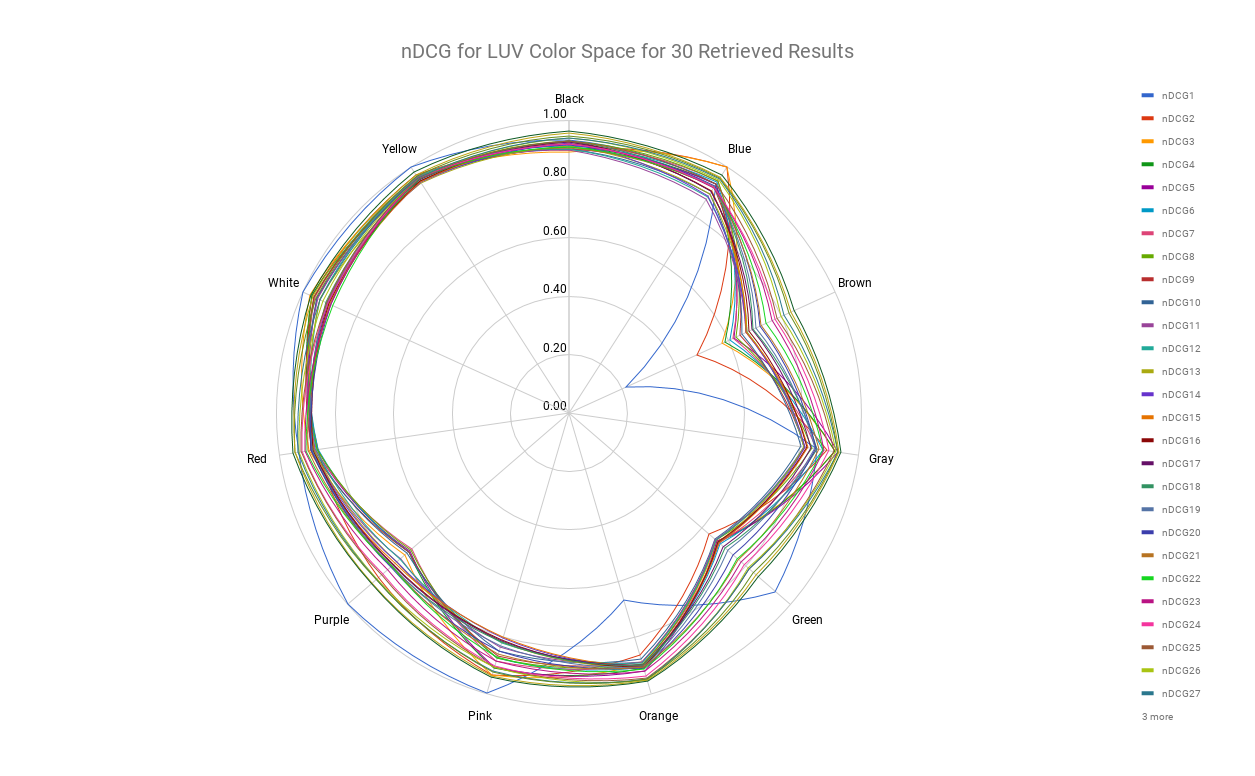
\includegraphics[width=0.9\linewidth]{image/retrievalTwo/radar_ndcg_luv.png}\\
    (a) \textit{nDCG} visualised in Radar Chart \\
    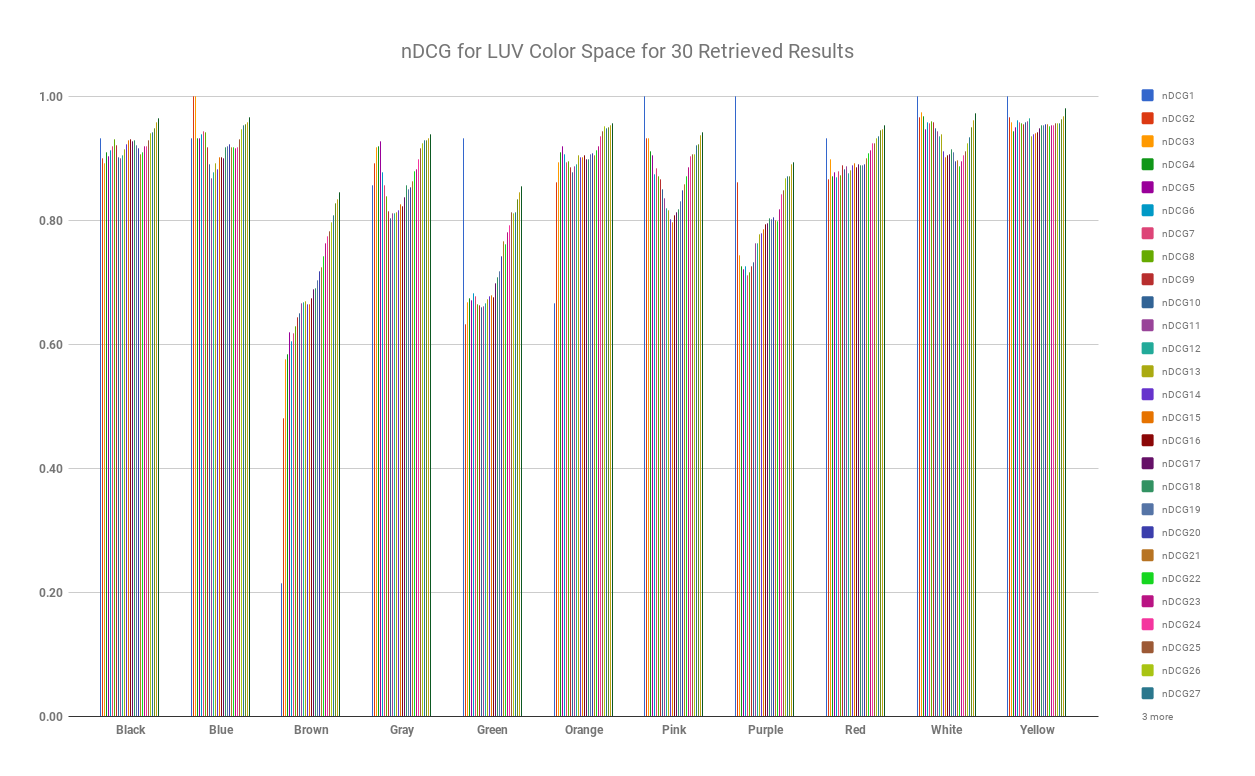
\includegraphics[width=0.9\linewidth]{image/retrievalTwo/bar_ndcg_luv.png}\\
    (b) \textit{nDCG} visualised in Bar Chart \\
  \end{tabular}
  \caption{\textit{nDCG} of the LUV Colour Mode using Radar and Bar Chart}
  \label{fig:colorndcg}
\end{figure}


\begin{table}[ht!]
	\centering
	\caption{Normalised Discounted Cumulative Gain (nDCG) for the LUV colour metrics}
	\label{tab:dcgColor}
\resizebox{\textwidth}{!}{
\begin{tabular}{c||c|c|c|c|c|c|c|c|c|c|c}
& Black & Blue & Brown & Gray & Green & Orange & Pink & Purple & Red & White & Yellow \\ \hline \hline
\textit{nDCG1} & 0.93 & 0.93 & 0.21 & 0.86 & 0.93 & 0.67 & 1.00 & 1.00 & 0.93 & 1.00 & 1.00 \\
\textit{nDCG2} & 0.90 & 1.00 & 0.48 & 0.89 & 0.63 & 0.86 & 0.93 & 0.86 & 0.87 & 0.97 & 0.97 \\
\textit{nDCG3} & 0.89 & 1.00 & 0.58 & 0.92 & 0.67 & 0.89 & 0.93 & 0.74 & 0.90 & 0.97 & 0.96 \\
\textit{nDCG4} & 0.91 & 0.93 & 0.58 & 0.92 & 0.68 & 0.91 & 0.91 & 0.73 & 0.87 & 0.97 & 0.94 \\
\textit{nDCG5} & 0.90 & 0.93 & 0.62 & 0.93 & 0.67 & 0.92 & 0.90 & 0.72 & 0.88 & 0.95 & 0.95 \\
\textit{nDCG6} & 0.91 & 0.94 & 0.60 & 0.88 & 0.68 & 0.91 & 0.87 & 0.73 & 0.87 & 0.96 & 0.96 \\
\textit{nDCG7} & 0.92 & 0.94 & 0.62 & 0.86 & 0.68 & 0.89 & 0.88 & 0.71 & 0.88 & 0.96 & 0.96 \\
\textit{nDCG8} & 0.93 & 0.94 & 0.63 & 0.84 & 0.66 & 0.90 & 0.87 & 0.72 & 0.87 & 0.96 & 0.96 \\
\textit{nDCG9} & 0.92 & 0.92 & 0.64 & 0.82 & 0.66 & 0.89 & 0.87 & 0.73 & 0.89 & 0.96 & 0.96 \\
\textit{nDCG10} & 0.90 & 0.89 & 0.65 & 0.80 & 0.66 & 0.88 & 0.85 & 0.73 & 0.88 & 0.95 & 0.96 \\
\textit{nDCG11} & 0.90 & 0.87 & 0.67 & 0.81 & 0.66 & 0.89 & 0.84 & 0.76 & 0.89 & 0.94 & 0.96 \\
\textit{nDCG12} & 0.90 & 0.88 & 0.67 & 0.81 & 0.67 & 0.89 & 0.82 & 0.76 & 0.88 & 0.94 & 0.96 \\
\textit{nDCG13} & 0.91 & 0.89 & 0.67 & 0.81 & 0.67 & 0.91 & 0.82 & 0.78 & 0.88 & 0.94 & 0.94 \\
\textit{nDCG14} & 0.92 & 0.88 & 0.67 & 0.82 & 0.68 & 0.90 & 0.80 & 0.78 & 0.89 & 0.91 & 0.94 \\
\textit{nDCG15} & 0.93 & 0.90 & 0.67 & 0.83 & 0.68 & 0.90 & 0.80 & 0.79 & 0.89 & 0.90 & 0.94 \\
\textit{nDCG16} & 0.93 & 0.90 & 0.68 & 0.82 & 0.68 & 0.90 & 0.81 & 0.79 & 0.89 & 0.90 & 0.94 \\
\textit{nDCG17} & 0.93 & 0.90 & 0.69 & 0.84 & 0.70 & 0.90 & 0.81 & 0.80 & 0.89 & 0.91 & 0.95 \\
\textit{nDCG18} & 0.93 & 0.92 & 0.69 & 0.86 & 0.71 & 0.90 & 0.82 & 0.80 & 0.89 & 0.91 & 0.95 \\
\textit{nDCG19} & 0.92 & 0.92 & 0.70 & 0.85 & 0.72 & 0.91 & 0.83 & 0.80 & 0.89 & 0.91 & 0.95 \\
\textit{nDCG20} & 0.92 & 0.92 & 0.72 & 0.85 & 0.74 & 0.91 & 0.85 & 0.80 & 0.89 & 0.89 & 0.96 \\
\textit{nDCG21} & 0.91 & 0.92 & 0.72 & 0.86 & 0.77 & 0.90 & 0.86 & 0.80 & 0.90 & 0.90 & 0.95 \\
\textit{nDCG22} & 0.91 & 0.92 & 0.74 & 0.88 & 0.76 & 0.91 & 0.87 & 0.80 & 0.91 & 0.89 & 0.95 \\
\textit{nDCG23} & 0.92 & 0.92 & 0.76 & 0.88 & 0.78 & 0.92 & 0.89 & 0.82 & 0.91 & 0.90 & 0.95 \\
\textit{nDCG24} & 0.92 & 0.92 & 0.77 & 0.90 & 0.79 & 0.94 & 0.90 & 0.84 & 0.92 & 0.90 & 0.95 \\
\textit{nDCG25} & 0.93 & 0.93 & 0.78 & 0.92 & 0.81 & 0.94 & 0.91 & 0.85 & 0.93 & 0.91 & 0.96 \\
\textit{nDCG26} & 0.94 & 0.95 & 0.80 & 0.92 & 0.81 & 0.95 & 0.91 & 0.87 & 0.93 & 0.93 & 0.96 \\
\textit{nDCG27} & 0.94 & 0.95 & 0.81 & 0.93 & 0.81 & 0.95 & 0.92 & 0.87 & 0.94 & 0.93 & 0.96 \\
\textit{nDCG28} & 0.95 & 0.96 & 0.83 & 0.93 & 0.83 & 0.95 & 0.92 & 0.87 & 0.95 & 0.95 & 0.96 \\
\textit{nDCG29} & 0.96 & 0.96 & 0.83 & 0.93 & 0.85 & 0.95 & 0.94 & 0.89 & 0.95 & 0.96 & 0.97 \\
\textit{nDCG30} & 0.96 & 0.97 & 0.85 & 0.94 & 0.85 & 0.96 & 0.94 & 0.89 & 0.95 & 0.97 & 0.98 \\
\end{tabular}}
\end{table}


\subsubsection{Retrieval Speed}

As with any retrieval engine, the speed of the retrieval engine plays an
important role in determining the feasibility of the proposed method. In this
experiment, the relevance of each result was not taken into consideration.
Instead, the time taken to perform the queries were measured. A baseline (BL)
measurement of the proposed method was performed with the default values of:
(i) Retrieval of 30 results, (ii) Trajectory length of 10 atoms, (iii) Includes
all colours and (iv) Sorting of first 200 Colour Matches (SortColourSize).
Using the BL setting, the proposed method ignores all colour information during
the retrieval process as only the trajectory information along with the time
and date input affects the final results.

Table \ref{tab:retrievalspeed} summarises the retrieval speed of the proposed
method using various settings. The collection of results were done by repeating
and averaging out 20 executions of queries. The results of the BL is highlighted
in the table. From the results, it is observed that the BL settings achieved an
average of 1.24 seconds when retrieving 30 results given an input trajectory of
10 atoms. The results also shows that increasing the number of displayed
results does not heavily affect the processing time. However, it is noticed
that the length of input trajectory affects the processing speed more than the
number of displayed results. This is consistent with the formula used to obtain
Chamfer Distance (see Eq. \ref{eq:chamferDistance}). As the length of the
queries increase, the proposed method would have to spend more time running
through each item within the set.

To further test the retrieval speed, colour information was given as an input.
With that, the proposed method took considerably more time than the BL
measurement. This is because the proposed method had to compare more data and
sort the returned results in accordance to both the colour accuracy as well as
the similarity between the input trajectory and the database records. In the
same manner, when the number of desired colours increased from 1 to 5, the
retrieval engine took an extra 0.3 seconds to process the results.

Next, to further validate the performance of the proposed method, synthetic
data was generated to simulate 6 months of valid data within the database.
When the BL settings were applied, the proposed method took 7.7 seconds to
retrieve the results. The additional colour queries only took an extra 0.6
seconds for the retrieval of results. Furthermore, the combination of input
trajectory length of 30 along with 5 colour queries only took 9.4 seconds for
the proposed method to produce the final results. When comparing against the
traditional method of manually filtering the data, the proposed method shows
significant improvement. Without a doubt, the proposed solution is able to
outperform any human. The comparison between the proposed method against the
method proposed by \citeA{castanon2016retrieval} is listed in
Table \ref{tab:compareresult}. Given the difference in the dataset used, it is
difficult to compare the methods used. Even though the proposed method was not
able to obtain high compression rates, it was able to search through 200 hours
of data within 1.2 seconds. This kind of efficiency is essential when dealing
with huge datasets.


% Please add the following required packages to your document preamble:
% \usepackage[table,xcdraw]{xcolor}
% If you use beamer only pass "xcolor=table" option, i.e. \documentclass[xcolor=table]{beamer}
\begin{table}[!tb]
	\centering
	\caption{Retrieval Speed with Varying Parameters}
	\label{tab:retrievalspeed}
	\resizebox{1\textwidth}{!}{
\begin{tabular}{|c|c|c|c|c|c|}
\hline
\textbf{Data Size} & \textbf{Result Size} & \textbf{Traj. Length} & \textbf{No. of Colours} & \textbf{SortColourSize} & \textbf{Avg Retrieval Speed } \\ \hline
\multicolumn{1}{|c|}{}            & \cellcolor{yellow}30                           & \cellcolor{yellow}10                         & \cellcolor{yellow}11                         & \cellcolor{yellow}200                     & \cellcolor{yellow}1246.7720 ms (BL)                        \\ \cline{2-6}
\multicolumn{1}{|c|}{}            & 30                           & 10                         & 1                         & 200                     & 1382.6237 ms                             \\ \cline{2-6}
\multicolumn{1}{|c|}{}            & 30                           & 30                         & 11                         & 200                     & 1301.3777  ms                           \\ \cline{2-6}
\multicolumn{1}{|c|}{}            & 100                          & 10                         & 11                         & 200                     & 1282.0485 ms                            \\ \cline{2-6}
\multicolumn{1}{|c|}{}            & 30                           & 10                         & 11                         & 500                     & 1374.3655 ms                             \\ \cline{2-6}
\multicolumn{1}{|c|}{}            & 30                           & 10                         & 1                          & 500                     & 1580.7543 ms                            \\ \cline{2-6}
\multicolumn{1}{|c|}{}            & 30                           & 30                         & 1                          & 500                     & 1641.2180 ms                            \\ \cline{2-6}
\multicolumn{1}{|c|}{\multirow{-8}{*}{1 month}}            & 30                           & 10                         & 5                          & 500                     & 1972.2770 ms                            \\ \hline \hline
\multicolumn{1}{|c|}{}           & \cellcolor{yellow}30                           & \cellcolor{yellow}10                         & \cellcolor{yellow}11                         & \cellcolor{yellow}200                     & \cellcolor{yellow}7745.1803 ms                            \\ \cline{2-6}
\multicolumn{1}{|c|}{}          & 30                           & 10                         & 1                          & 200                     & 7874.1965 ms                            \\ \cline{2-6}
\multicolumn{1}{|c|}{}           & 30                           & 10                         & 5                          & 200                     & 8314.7145 ms                            \\ \cline{2-6}
\multicolumn{1}{|c|}{\multirow{-4}{*}{6 month}}           & 30                           & 30                         & 5                          & 200                     & 9369.6657 ms                            \\ \hline
\end{tabular}}
\end{table}

% Please add the following required packages to your document preamble:
% \usepackage[table,xcdraw]{xcolor}
% If you use beamer only pass "xcolor=table" option, i.e. \documentclass[xcolor=table]{beamer}
\begin{table}[]
	\centering
	\caption{Comparison between Methods: Retrieval Speed, Compression Ratio Using Trajectory/Tracklet Features}
	\label{tab:compareresult}
	\resizebox{\textwidth}{!}{
\begin{tabular}{|l|l|l|l|l|l|}
\hline
\textbf{Method}                 & \textbf{Video Duration} & \textbf{Video Size} & \textbf{DB/Index Size} & \textbf{Compression Ratio}        & \textbf{Retrieval Speed}         \\ \hline
DP + LSH
%\citeyear{castanon2016retrieval}
& 13.8 minutes                    & 1.16 GB             & 153 KB                       & 7581\%                            & 2.9 sec*                         \\ \hline
%\citeA{castanon2016retrieval}
DP + LSH & 13.8 minutes                    & 529 MB              & 65 KB                        & \cellcolor{yellow}8138.46\% & 4.32 sec*                        \\ \hline
Proposed method                      & 200 hours                       & 33.4 GB             & 16.3 MB                      & 2049.07\%                         & \cellcolor{yellow}1.2 sec** \\ \hline
\end{tabular}}
\end{table}



\section{Summary}

In this chapter, two different semantic retrieval engines were proposed to
retrieve semantics extracted in Chapter \ref{section:semanticsextraction}.
Both the proposed methods implements distinctly different algorithm for the
retrieval process. The \versionOneRet retrieved relevant documents based on the
locality in which the data was saved while the \versionTwoRet retrieved and
sorted relevant documents based on the similarity with the given input.

Both of the retrieval engine reported respectable precision when retrieving
both motion and colour information. The proposed \versionTwoRet also
demonstrates its ability to retrieve relevant results accurately within 1.2
seconds while organising the results in the best possible manner. Along with
that, as the colour semantics were not hard coded into one final category,
the colour retrieval process shows significant improvement over the method
proposed in \versionOneRet.

